\chapter{Results and Discussion} \label{ch_result}
We described a mathematical model for electroconvection of conductive fluid in a thin annular region. From its description in~(\ref{dim_less_1})--(\ref{dim_less_end}), the flow can be characterized by a small set of nondimensional parameters that reflect the geometry, $\alpha$, the fluid properties $(\mathcal{P}, \mathrm{Re})$ and with the strength of an external imposed electric field, (the Rayleigh number $\mathcal{R})$.

For a given experiment with a fixed geometry, the details of the flow vary as the potential difference across the fluid is varied. If the voltage difference is very low then the fluid flow is axisymmetric. As the voltage difference is increased, at some point, the character of the fluid flow changes. Beyond this point, further increases  of the voltage difference lead to more complex flow patterns.

In this chapter, we will study how the model reflects these experimentally observed changes through variation in the Rayleigh number $\mathcal{R}$. We have implemented a matrix-free numerical bifurcation method in MATLAB that traces two types of compact invariant limit sets (steady states and limit cycles) of the continuous dynamical system~(\ref{eq_gen_dy_sys}). This method is employed to compute and detect steady flows and transition points in the sheared annular electroconvection problem as the dimensionless Rayleigh number $\mathcal{R}$ is varied.
The implemented method consists of computing fixed points of two types of a discrete dynamical system. These fixed points correspond to the two different types of limit sets (steady states, limit cycles) of the continuous dynamical system.

The steady states of the continuous system, that correspond to the base state (axisymmetric flow) in the physical system, are obtained by computing fixed points $(\mathbf{u},\mathcal{R})$ of the discrete dynamical system~(\ref{fixed_point_map}), where $\mathbf{u}$ is an $n$-dimensional vector that consists of the discretized perturbations from the base state of the four dynamic physical quantities of annular electroconvection ($\psi_2$: the electric potential; $q$: the charge density; $\omega$: the vorticity; $\phi$: the streamfunction).
Limit cycles, which correspond to a rotating wave in the physical system, are computed using the approach described in Section~\ref{sc_ti_ap}. Using this approach, limit cycles in the continuous system are computed as fixed points $(\mathbf{u},w,\mathcal{R})$ of the discrete dynamical system~(\ref{rel_eqi_1}), where $w$ is the phase speed of the periodic solution.

\begin{figure}[t]
\centerline{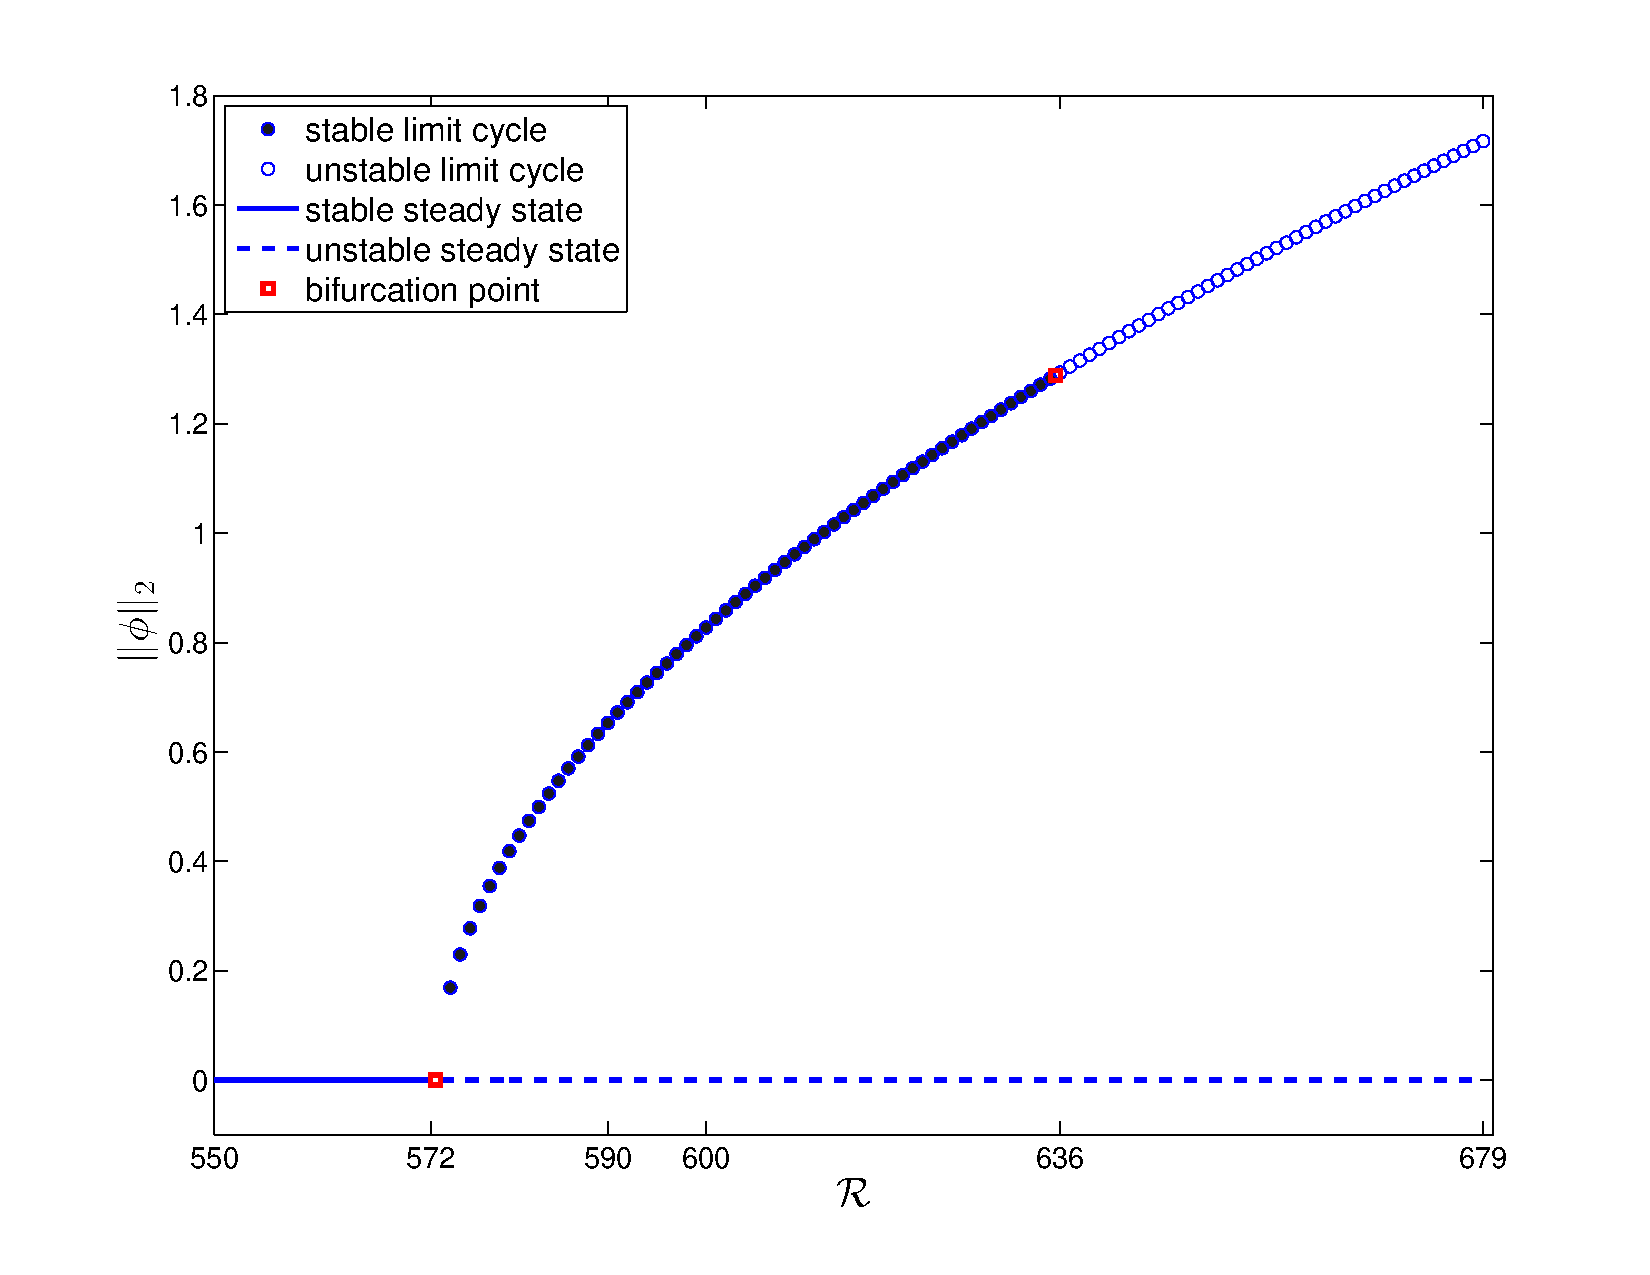
\includegraphics[width = .9\textwidth]{./figures/Pictures/Bifurcation_Diagram.pdf}}
\caption{A bifurcation diagram illustrating the 2-norm of perturbations of the streamfunction $\phi$ from the axisymmetric flow as the Rayleigh number is varied.  The other dimensionless parameters of the experiment are fixed to  $\mathcal{P} = 75.8, \mathrm{Re} = 0.249, \alpha = 0.56$. }
\label{bif_diag}
\end{figure}

The main parameter of interest with respect to the dynamics is the Rayleigh number $\mathcal{R}$. We fix the other parameters of as in~\cite{PeiChunTsain}; they are listed in Table~\ref{table_para} under the model parameters.
The results obtained using the methods described in this thesis are compared to the current literature~\cite{DNSSAE,PeiChunTsain}, where in contrast with this thesis work, the equilibrium flows and the transitions are identified by applying random initial conditions to numerical simulations of the perturbation equations with relatively long integration time.

The primary result of this thesis is depicted in the bifurcation diagram in Figure~\ref{bif_diag}. Using the matrix-free numerical bifurcation method, two solution curves are traced by varying the Rayleigh number $\mathcal{R}$---the zero solution curve corresponds to the axisymmetric flow, while the other curve corresponds to a rotating wave flow. A primary bifurcation is detected at a critical Rayleigh number $\mathcal{R}_c = 572$ at which the flow exhibits a transition from the base state (axisymmetric flow) to rotating waves. Figure~\ref{axi2rot} illustrates the flow pattern that the fluid exhibits before and after the primary transition.
Beyond this transition, we detect that a secondary bifurcation from rotating waves occurs at $\mathcal{R}_c = 636$. A further discussion of these results is developed in the subsequent sections. For each of the identified flow patterns, the secondary parameters remain the same.

Each technique itself requires a set of numerical parameters. These values have also been collected into Table~\ref{table_para} for convenience. In the section that follows, the details of the computation and the results obtained are presented and compared to the results revealed in previous experimental, analytical~\cite{linearstability} and numerical~\cite{SBSAE,PeiChunTsain} results found in the literature.
%%%%%%%%%%%%%%%%%%%%%%%%%%%%%%%%%%%%%%%%%%%%%%%%%%%%%%%%%%%%%%%%%%%%%%%%%%%%%%%%%
\begin{figure}[t]
\centerline{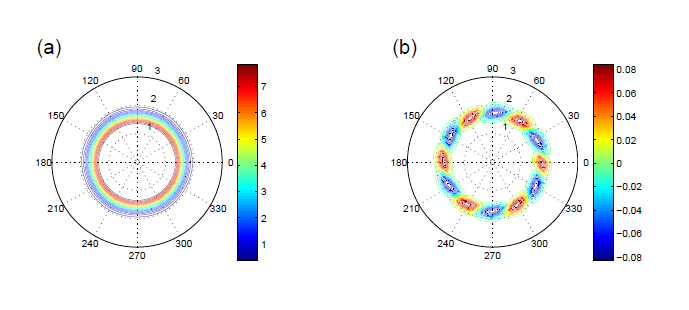
\includegraphics[width= .9\textwidth]{./figures/Pictures/axi_rot_plot.png}}
%\vspace{-3cm}
\caption{The (a) axisymetric and (b) rotating waves flow patterns at the onset of convection.}
\label{axi2rot}
\end{figure}

\begin{table}[bth]
\begin{center}
\caption{The nominal parameters used in the numerical results.\label{table_para}} \begin{tabular}{l|p{8cm}|l} \hline\hline\multicolumn{3}{c}{Model parameters}\\
\hline Symbol & Parameter & Value \\ \hline
$\mathcal{P}$ & Prandlt number & 75.8\\
$\mathrm{Re}$ & Reynolds number &  0.249\\
$\alpha$ & Aspect ratio &  0.56\\ \hline
\multicolumn{3}{c}{Time stepper: discretization parameters}\\ \hline
 Symbol & Parameter & Value \\ \hline
 $N_c$ &  Highest order of the Tchebychev basis & 24\\
 $K$  & Highest Fourier wave number & 32 \\
$\delta t$ &   Time step  & $5\times10^{-4}$\\
\hline \multicolumn{3}{c}{Numerical bifurcation parameters}\\ \hline
 Symbol & Parameter & Value \\ \hline
 \texttt{ds}  & Step size in the parameter space: & \\
	& First transition; Second transition & $1$; $\pm 1$\\
$t$ & Arbitrary integration time  & $0.2$ \\
 $\epsilon$ & Perturbation amplitude of the forward finite difference approximation &  $10^{-3}$\\
\texttt{Kmax} & Maximum number of iteration of Newton-Raphson   & $50$\\
\texttt{New\_res}& Newton-Raphson residual tolerance:  & \\
	& First transition; Second transition & $10^{-8}$; $10^{-6}$\\
\texttt{gmres\_tol} & GMRES tolerance & $10^{-4}$\\ \hline\hline
 \end{tabular} \end{center} \end{table}

\section{Transition from axisymmetric flow to rotating waves flow} \label{sec_axi2rot}
At a Rayleigh number of zero, there is no applied electric field and the flow is axisymmetric as previously mentioned. Gradually increasing the Rayleigh number $\mathcal{R}$ from zero, the flow transitions at a critical value $\mathcal{R}_c$ from axisymmetric to rotating waves. The zero solution curve corresponding to perturbations from the base state (axisymmetric) is traced out where we determine the bifurcation point at which the primary transition occurs.
The zero solution curve is traced out using the matrix-free numerical bifurcation method described in Section~\ref{sec_st_state} by computing a sequence of fixed points $\{(\mathbf{u}_i,\mathcal{R}_i)\}_{i=0}^{130}$ of the discrete dynamical system~(\ref{fixed_point_map}). These fixed points correspond to the steady states of the continuous dynamical system corresponding to the axisymmetric flow. Previous results~\cite{PeiChunTsain} have shown that the primary transition occurs at $\mathcal{R}_c = 572$, and this was the main motivating factor to begin tracing the solution at $\mathcal{R}_0 = 550$. This also greatly reduce unnecessary computation for lower $\mathcal{R}$ where the flow remains axisymmetric. Typically, the initial state of the perturbation equations is set at some fixed point, say $(\mathbf{u}_0,\mathcal{R}_0) = (\boldsymbol{0},550)$, from which $\mathcal{R}$ is increased. The corresponding eigenvalue problem is solved to identify the local behaviour of the axisymmetric flow. In our implementation, we elect to acquire the initial fixed point by correcting the Newton-Raphson solver guess $(\hat{\mathbf{u}}_{0},\mathcal{R}_0)$ to within a residual error of $10^{-8}$. This initial guess $(\hat{\mathbf{u}}_{0},\mathcal{R}_0)$ is obtained by time integrating some random initial condition for $t = 5$ (10000 time steps) with the Rayleigh number fixed at $\mathcal{R}_{0} = 550$. The time integration gives a good approximation of the steady solution because for $\mathcal{R} < \mathcal{R}_c$, the perturbations from the base state decay rapidly in time. Note that this approach is not used extensively in this thesis. In particular, the only other time is used to obtain the initial nonlinear solver guess when computing solutions corresponding to the rotating waves.

Upon obtaining $(\mathbf{u}_0,\mathcal{R}_0)$, the solution curve is traced out as the Rayleigh number is varied up to $\mathcal{R} = 679$ with a unit step size. The parameters of the numerical bifurcation method are listed in Table~\ref{table_para}.
%The linear system at every Newton step is solved using GMRES with a relative residual set at $10^{-4}$. The perturbation amplitude of the forward finite difference approximation is set to $\epsilon = 10^{-3}$ and the evolution time of the map $\Phi_t$ (\ref{flow_map}) is fixed at an arbitrary choice $t = 0.2$.
The time of integration $t$ can be chosen arbitrarily and different choices $t = \{0.05,0.1,0.2\}$ were tested. %with the final time chosen small enough to resolve the flow but not so long as to exceed the GMRES tolerance.
It was found that the evolution time $t$ for the steady state solution did not affect the convergence of the linear solver as well as the eigenvalue solver. However for the more complicated invariant limit sets (limit cycle), the time-integration becomes crucial to the computation.

Upon obtaining these equilibrium flows, a linear stability analysis is performed to identify their local behaviour. In particular, the ten largest magnitude eigenvalues $\lambda$ of the linearization $\mathrm{D}_{\mathbf{u}}\Phi_t$ of the map are computed using the Implicitly Restarted Arnoldi method as implemented in the MATLAB function \texttt{eigs}. The integration-time of the map $\Phi$ is also set at $t = 0.2$. This relatively long integration time aids in clustering the spectrum because the system is dissipative, and thus improves the convergence properties. The results presented in Figure~\ref{eig_axi_rot}, show that a complex conjugate pair of eigenvalues crosses  the unit circle at a critical Rayleigh number $\mathcal{R} = 572$, i.e. for $\mathcal{R} <572$ all eigenvalues have modulus less then 1 and for $\mathcal{R} > 572$ at least one pair of complex eigenvalues has modulus greater than 1. The type of this bifurcation is known as a {Neimark-Sacker} bifurcation of the map, and, in particular, a supercritical {Neimark-Sacker}, because at the bifurcation point, the fixed point changes stability and co-exists with a stable isolated closed invariant curve~\cite{Kuznet}.

\begin{figure}[t]
\centerline{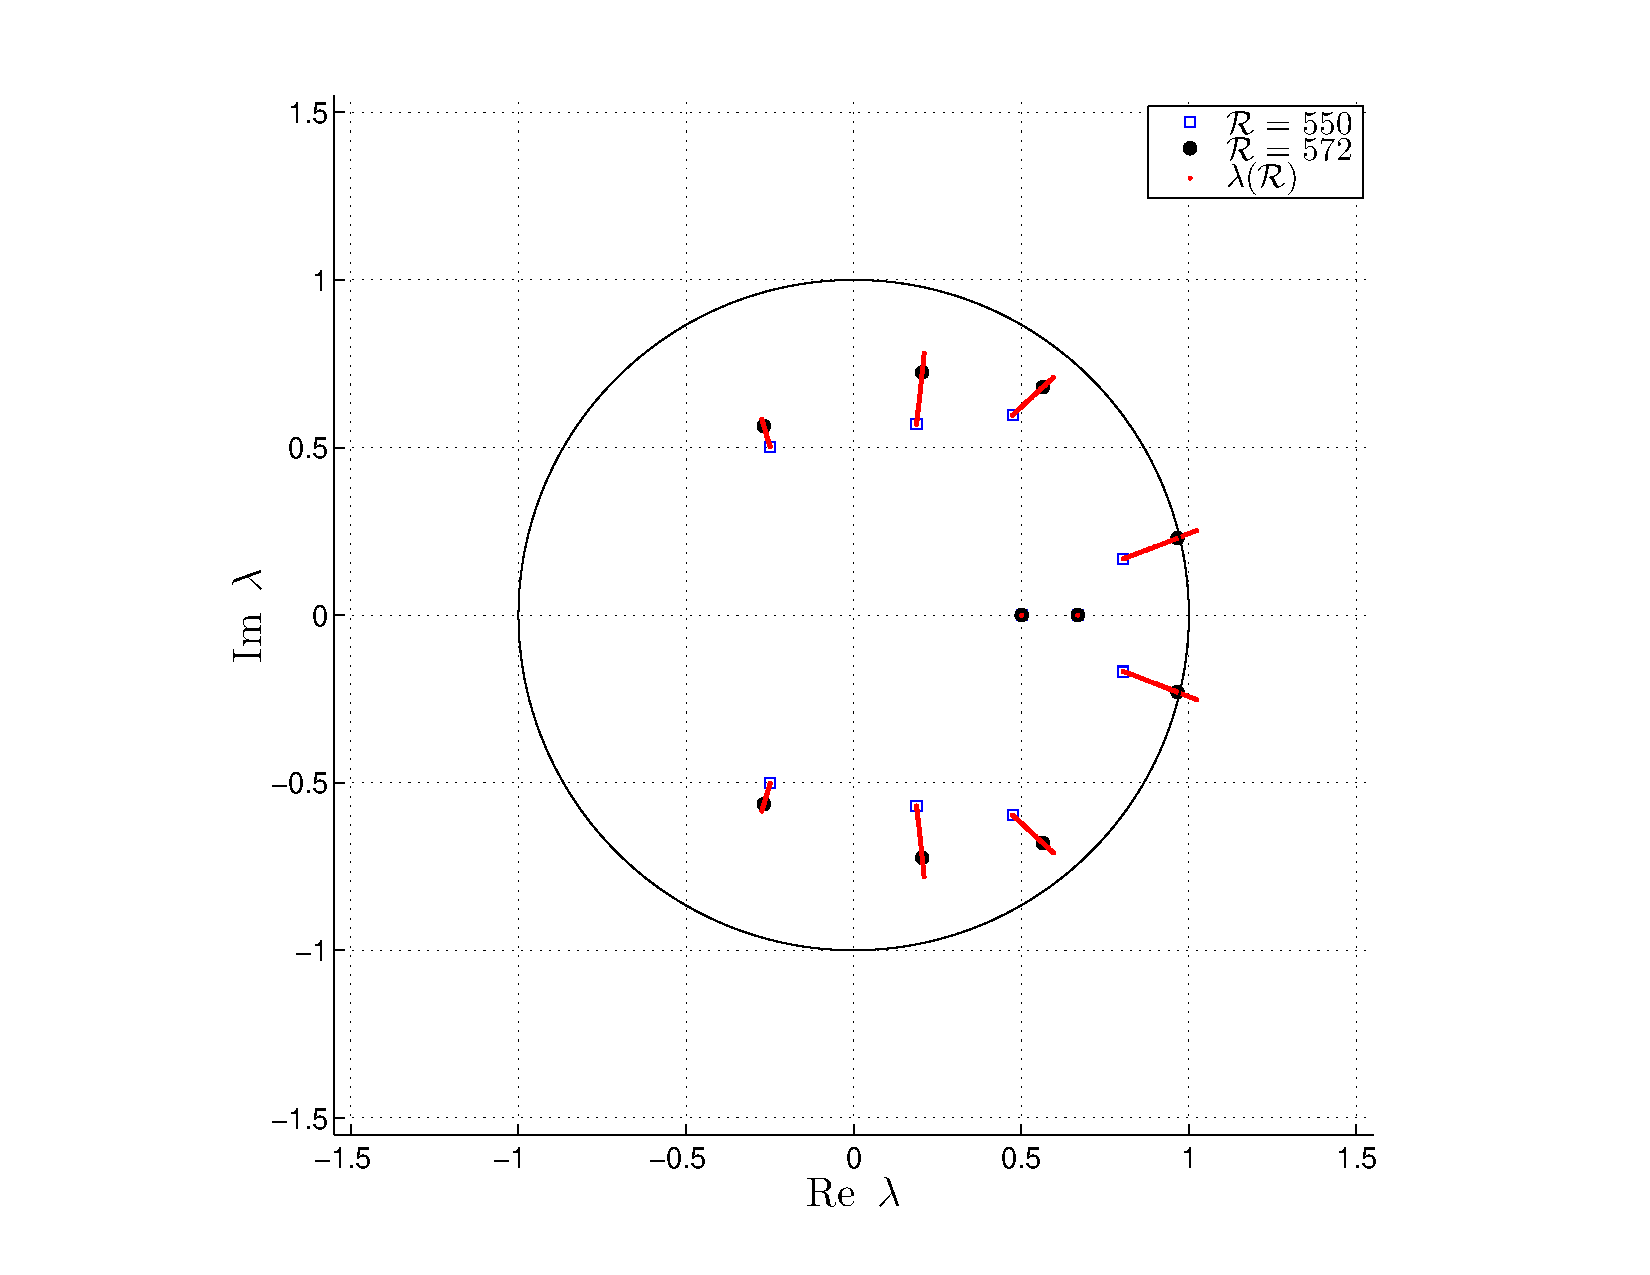
\includegraphics[width = 0.9\textwidth]{./figures/Pictures/Eigenvalue_axi_perio}}
\caption{The evolution of the eigenvalues of largest modulus corresponding to the  linearization of the map $\Phi$ about the solution $\mathbf{u}$. Only the largest 10 are depicted.}
\label{eig_axi_rot}
\end{figure}

\subsection{Interpretation and validation}
In the physical experiment, upon rotating the inner boundary at a constant speed $\omega_{i}$ and gradually increasing the electric potential difference $V$, a primary transition occurs from axisymmetric flow to rotating wave flow. In terms of the dimensionless parameters, varying the electric potential $V$ corresponds to varying the Rayleigh number $\mathcal{R}$. Direct numerical simulation has been performed in~\cite{PeiChunTsain} for the same set of dimensionless parameters listed in Table~\ref{table_para} as the Rayleigh number $\mathcal{R}$ is varied. In these simulations, it was found that a primary transition occurs at $\mathcal{R}_c = 572$ from axisymmetric to rotating waves at which the flow consists of six pairs of the counter rotating vortices. This bifurcation was observed to be a supercritical Hopf bifurcation~\cite{DNSSAE,PeiChunTsain}. These results are in agreement with the linear stability analysis performed in~\cite{linearstability} which predicted that the primary transition is a supercritical Hopf bifucation.

In summary, the results obtained using the matrix-free numerical bifurcation method described in this thesis are in agreement with previous results, with a supercritical Neimark-Sacker bifurcation of the discrete dynamical system identified at $\mathcal{R}_c = 572$, which corresponds to a supercritical Hopf bifurcation in the corresponding continuous dynamical system. At this bifurcation, the eigenfunction associated with the critical eigenvalue has an azimuthal mode of $m_c = 6$.


\section{Transition from rotating waves flow to amplitude vacillation}\label{sec_rot2ampv}
If $\mathcal{R}$ is increased beyond $\mathcal{R}_c = 572$, a secondary flow transition can be detected. In this section, we present the computational details involved in tracing out the solution curve corresponding to a flow of rotating waves, and in pinpointing, for the first time, a secondary bifurcation point. Using numerical simulations, we show that the flow transitions to amplitude vacillating waves and we validate these results, by comparing it to previous observations and analysis.
The solution curve corresponding to the rotating wave flow is constructed by computing a sequence of fixed points $\{(\mathbf{u}_i,w_i,\mathcal{R}_i)\}$ of the discrete dynamical system~(\ref{fixed_point_map}) with the technique described in Section~\ref{rel_equ}. Specifically, the rotating wave is considered as a relative equilibrium and is computed by determining its phase speed $w$. This differs from the more common approach of computing the flow as a limit cycle.
\begin{figure}[t]
\centerline{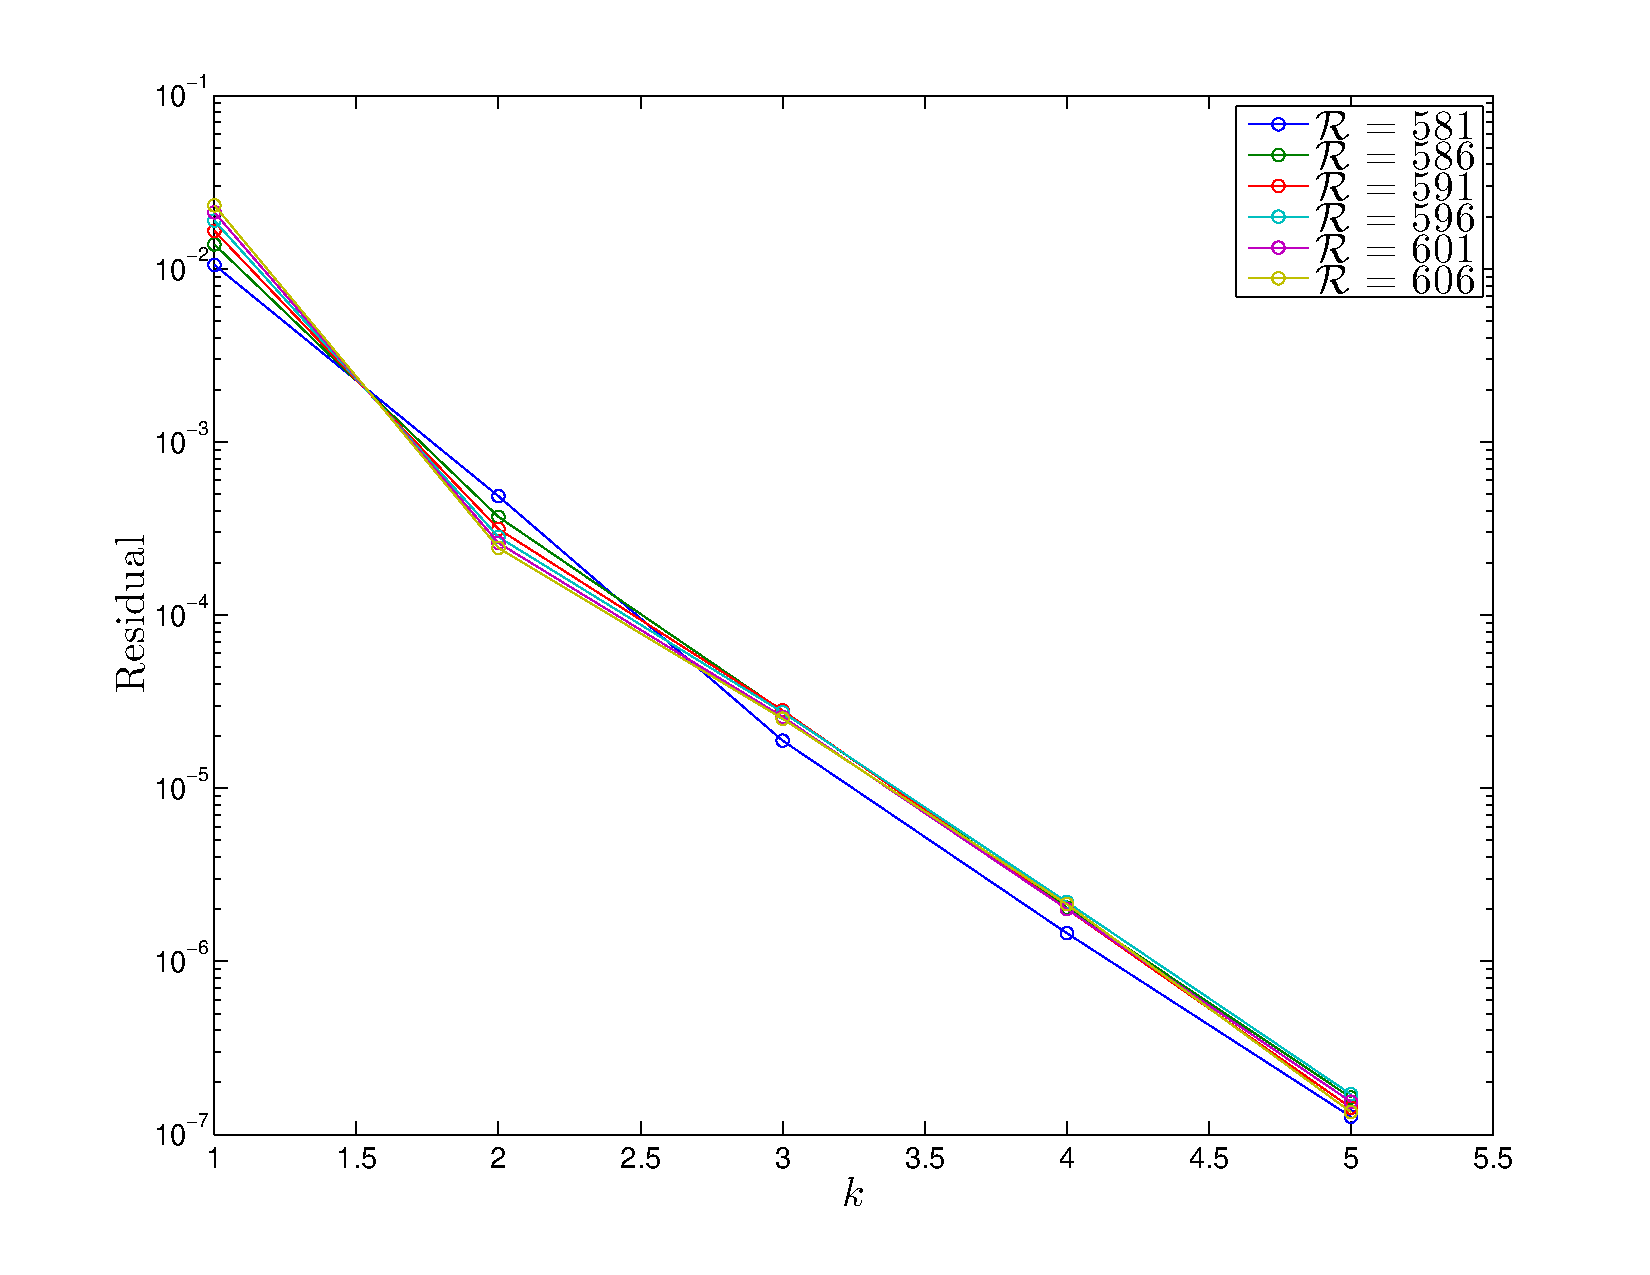
\includegraphics[width = 0.9\textwidth]{./figures/Pictures/Newton_residual}}
\caption{Convergence rate of the Newton residual as a function of iteration number $k$ of the refinement process. }
\label{New_conv}
\end{figure}

We set the parameters of the matrix-free numerical bifurcation method as listed in Table~\ref{table_para}. The solution curve is then traced out from an initial solution $(\mathbf{u}_0,w_0,\mathcal{R}_0)$ obtained by correcting an initial guess,
$\mathrm{\hat{X}}^{(0)} = [\mathbf{\hat{u}}^{(0)};\hat{w}^{(0)}]$,
using a Newton-Raphson solver within the desired residual tolerance of $10^{-6}$. The superscript denotes the iteration of the nonlinear solver. The initial phase speed guess of the rotating waves is set to an arbitrary value $\hat{w}^{(0)} = \pi/6$ and $\mathbf{\hat{u}}^{(0)}$ is obtained as before, by time stepping some random initial condition for a relatively long time $t = 10$ (20000 time steps) but in this case, with $\mathcal{R} = 580 > \mathcal{R}_c$. At this parameter value the solution associated with the flow of rotating waves is stable and the time integration is sufficient to remove any transients in the flow patterns.

The initial guess vector $\mathrm{\hat{X}}^{(0)} = [\mathbf{\hat{u}}^{(0)};\hat{w}^{(0)}]$ is corrected using the Newton-Raphson nonlinear solver which yields an $\mathrm{X}^{(k)} = [\mathbf{u}^{(k)};{w}^{(k)}], k = 1,2,\cdots,\texttt{Kmax}$, with $\mathcal{R} = 580$. The branch of solutions is then traced out by increasing the Rayleigh number $\mathcal{R} = 580$ up to $\mathcal{R} = 679$, with a unit step size  and then back down to the primary bifurcation point at $\mathcal{R}_c = 572$.
During this process, the nonlinear solver and the linear solver are observed to converge within the desired tolerance. Figure~\ref{New_conv} shows the convergence of the nonlinear solver for the rotating wave solution. The 2-norm of the residual is plotted on a log scale with respect to the iteration number.

\begin{figure}[t]
\centerline{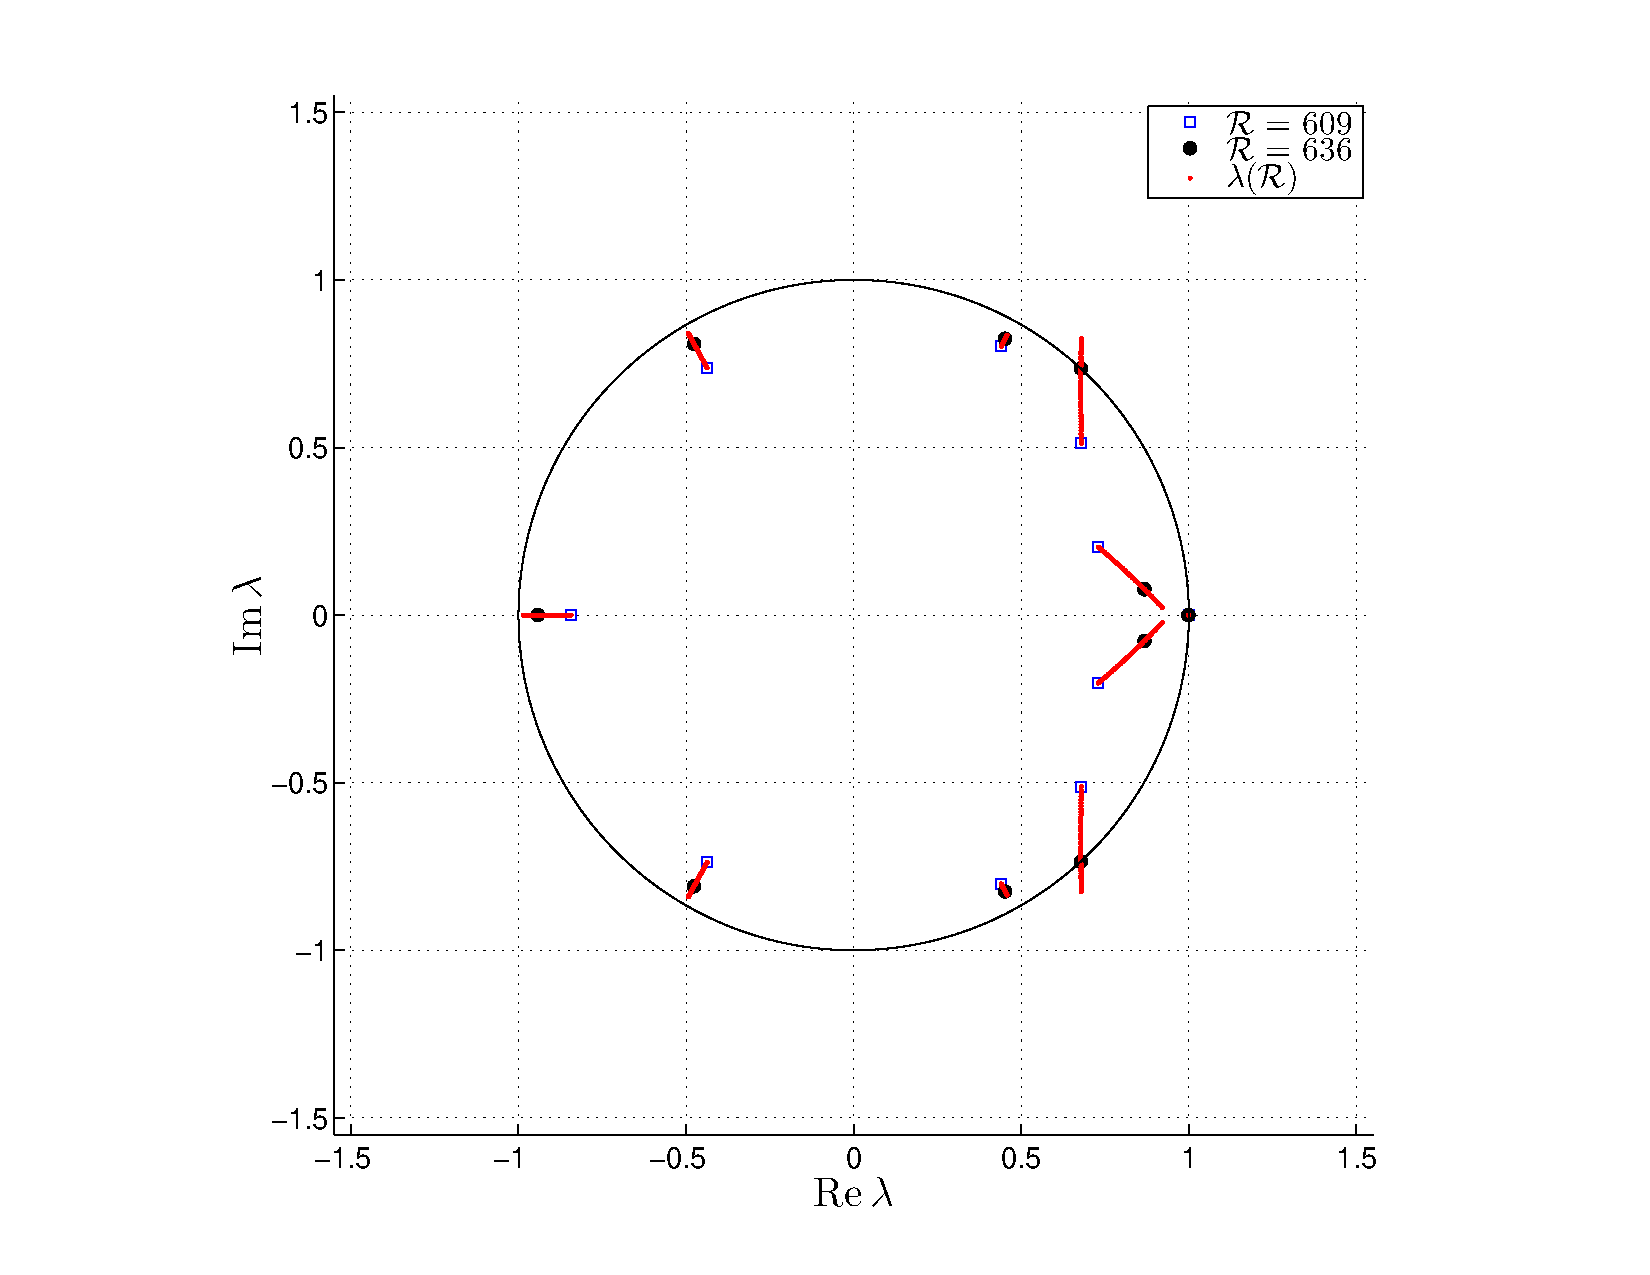
\includegraphics[height = 12cm, keepaspectratio]{./figures/Pictures/Eigenvalue_period_torus}}
\caption{The evolution of the eigenvalues of the linearization of the map $\Phi_\tau$ corresponding to the rotating waves flow. As in Figure~\ref{axi2rot} only the 10 largest with respect to modulus are depicted.}
\label{eig_rot_torus}
\end{figure}

Upon obtaining these fixed points of the map, the eigenvalue problem is solved to identify the local behaviour of these periodic solutions. To solve the eigenvalue problem, the period $\tau$ is computed using~(\ref{period_comp}) and found to be in the range of $0.1928 \le\tau\le 0.1933$, for $573\le\mathcal{R}\le 679$.

At $\mathcal{R}_{c_2}= 636$, a complex conjugate pair of eigenvalues of the linearization $\mathrm{D}_{\mathbf{u}}\phi_\tau$ of the map crosses the unit circle; see Figure~\ref{eig_rot_torus}.  Thus, for $572 < \mathcal{R} < 636$, the solution corresponding to the rotating waves is asymptotically stable, and unstable for $\mathcal{R} \ge 636$, and a {Neimark-Sacker} bifurcation is detected at $\mathcal{R} = 636$.

We may be able to gain insight into the type of flow transition to which this bifurcation corresponds by looking at the eigenfunctions corresponding to these eigenvalues.  In particular, if the bifurcation is non-degenerate, then it is expected that, to first order, the bifurcating flow will be a superposition of the original rotating wave and a perturbation whose amplitude grows from zero as the parameter varies through the bifurcation point, and whose features can be approximated from the eigenvalues and eigenfunctions.  Specifically, in this case, the perturbation will be a rotating wave whose phase speed can be approximated from the imaginary part of the eigenvalues, and whose spatial form can be approximated from the eigenfunctions.  The form of the eigenfunction corresponding to the critical eigenvalues can be seen in Figure~\ref{eigenfuntion}, i.e. it is a wave of mode $m_{c_2} = 6$, i.e. it has six pairs of counter rotating vortices just like the original rotating wave.  Thus, the bifurcating flow is expected to resemble a superposition of two rotating waves that have the same azimuthal wave number, but different phase speeds, i.e. an amplitude-modulated, or an \emph{amplitude vacillating}, wave.

However, based on the information at hand, we do not know whether the bifurcating flow is stable or unstable, or, alternatively whether the bifurcation is supercritical or subcritical.  It may be possible to determine this by computing the appropriate normal form coefficients.  However, this computation is prohibitively intensive.  Therefore, in this thesis, we will use simulations to provide evidence of the stability of the flow, and leave the proof to future work.  We discuss these simulations further in the next section.


%A {Neimark-Sacker} bifurcation is detected  at $\mathcal{R}_{c_2} = 636$; see Figure~\ref{eig_rot_torus}, at which a pair of the linearization $\mathrm{D}_{\mathbf{u}}\phi_\tau$ of the map crosses the unit circle. This bifurcation corresponds to a transition from the rotating wave flow. The eigenfunctions corresponding to the unstable eigenvalue corresponding to the unstable eigenvalues is also a rotating wave with mode $m_{c_2} = 6$, six pair of counter rotating vortices, however travelling at a different phase speed as shown in Figure~\ref{eigenfuntion}. Because this bifurcation is nondegenerate, the solution we see to first order analysis, is a superposition of the rotating wave with a scalar multiple of the eigenfunction. This further indicates that the rotating wave will transition to an amplitude vacillating wave flow.
%However, at this point, the analysis has not determined to what the flow will transition.
%To further validate this analysis, we  simulate the solution corresponding to the rotating wave flow for the Rayleigh number $\mathcal{R}= 640$ with a perturbation on the order of $10^{-3}$, and we observe that the rotating wave flow transitioned to amplitude vacillating waves. We conclude that for $572 < \mathcal{R} < 636 $, the solution corresponding to the rotating waves flow is asymptotically stable, and unstable for $\mathcal{R} \ge 636$.
\begin{figure}[t]
\centering
\subfigure[][]{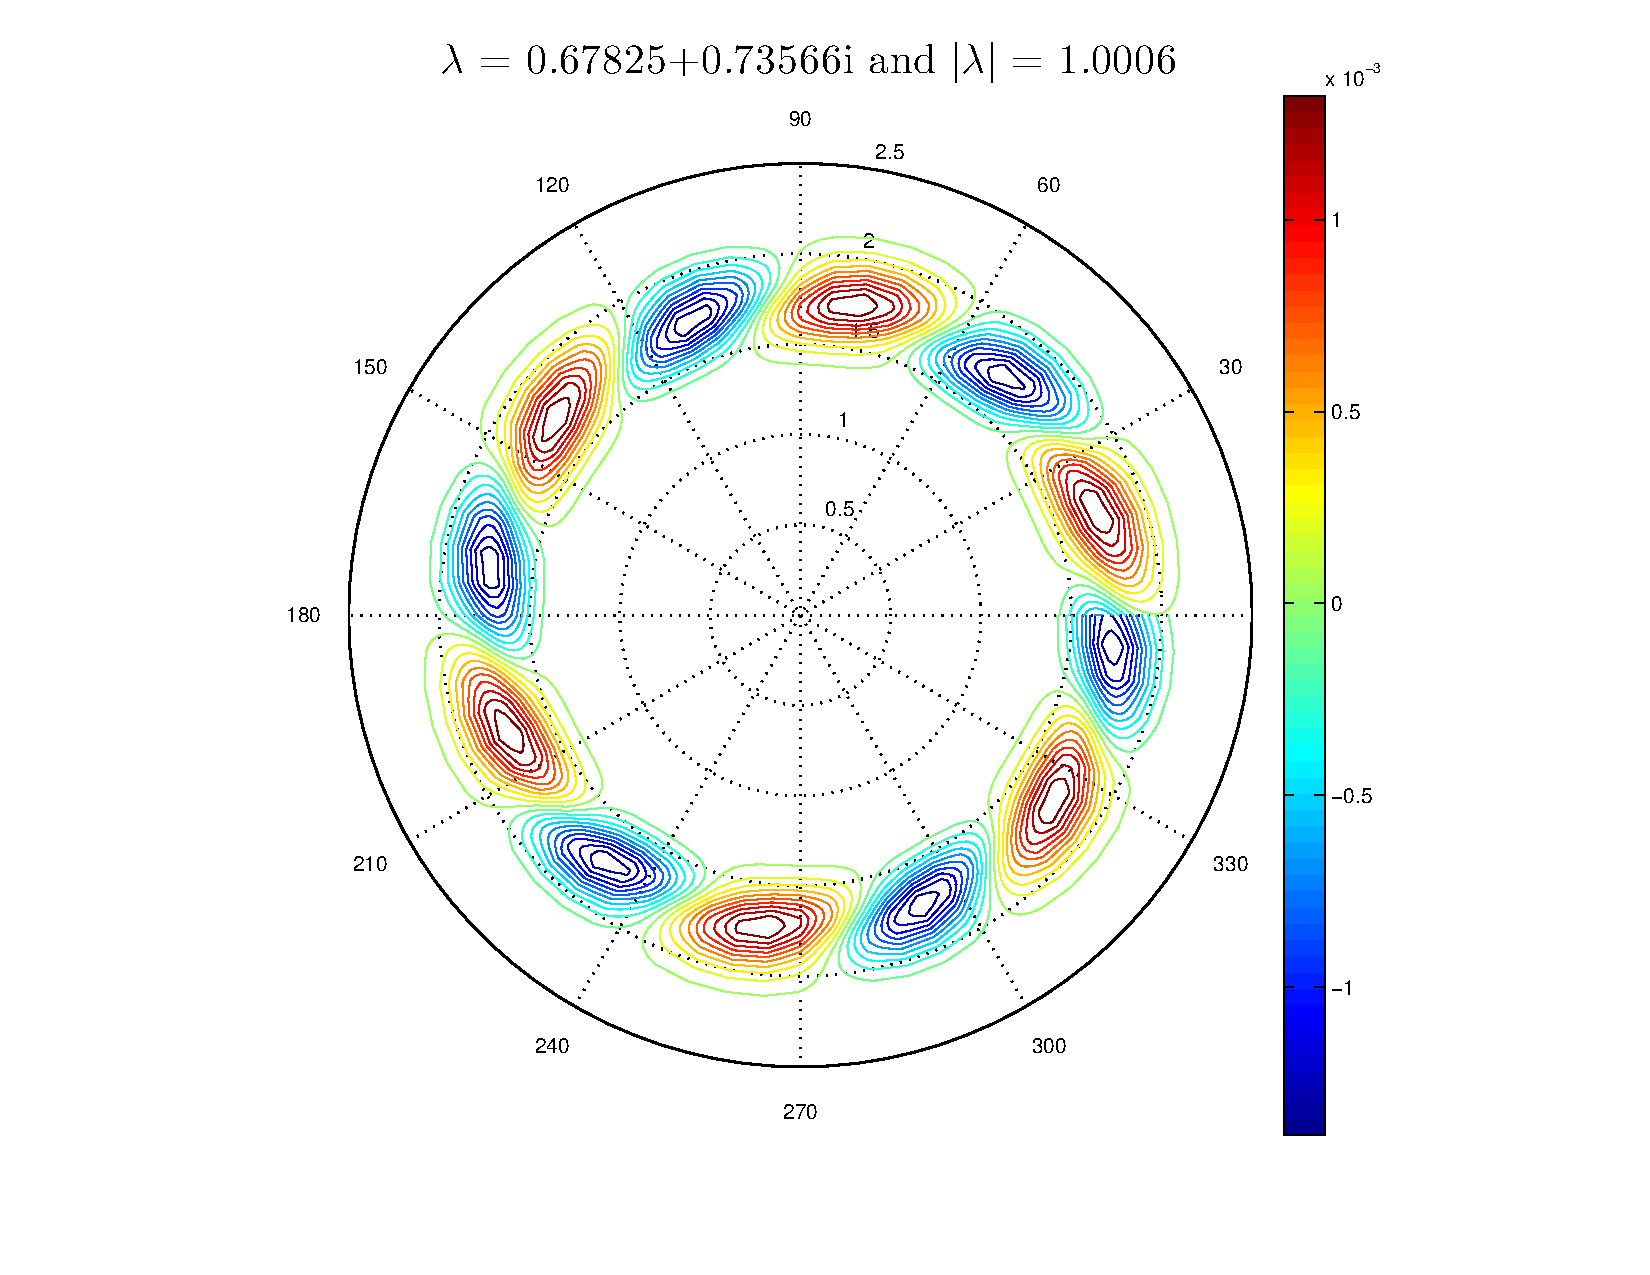
\includegraphics[width = 0.45\textwidth]{./figures/Pictures/Eigen_function_1}}
\hspace{8pt}
\subfigure[][]{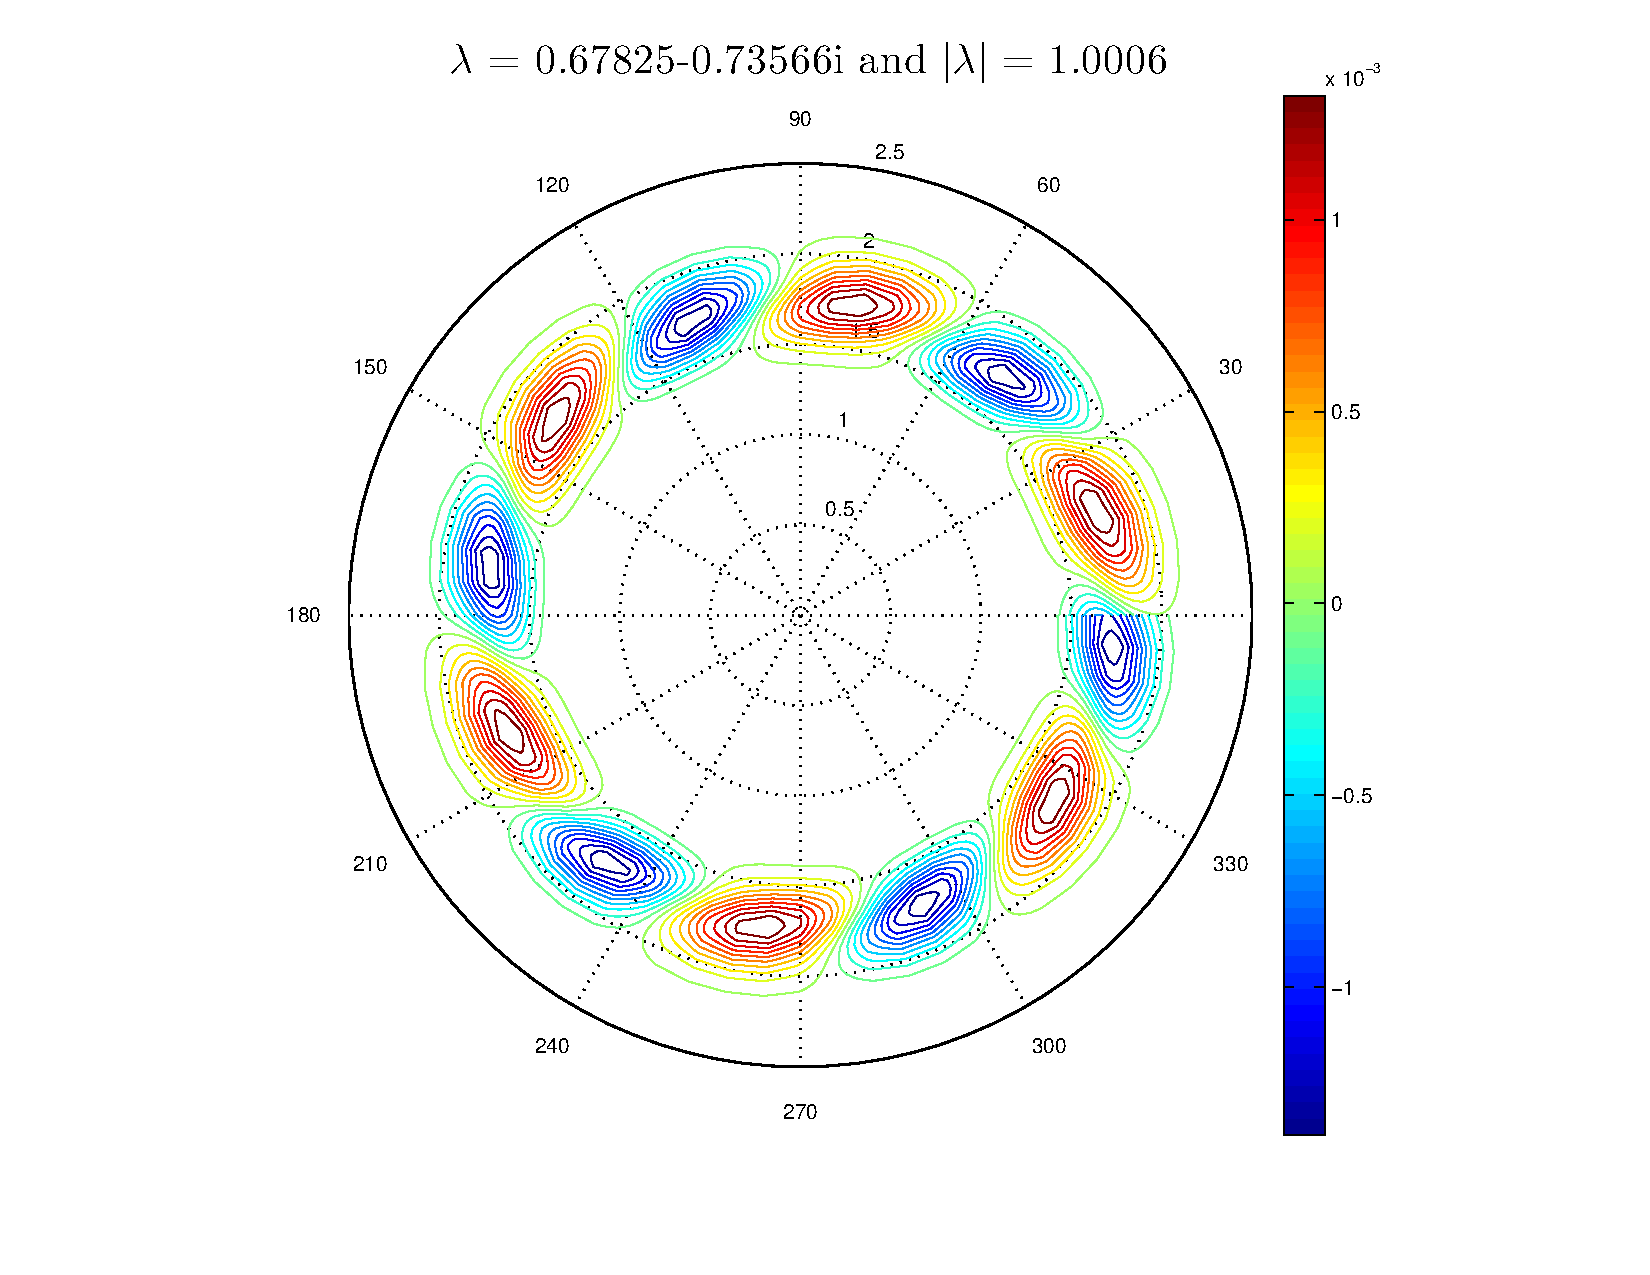
\includegraphics[width = 0.45\textwidth]{./figures/Pictures/Eigen_function_2}}
\hspace{8pt}
\caption{Real part of the eigenfunction of the streamfunction $\phi$  corresponding to the critical eigenvalues of the linearization $\mathrm{D}_{\mathbf{u}}\phi_{\tau}$ of the map.
\label{eigenfuntion}}
\end{figure}

\subsection{Interpretation and validation}
Beyond the primary transition, the physical experiment has a limited ability to visualize subsequent changes in the flow. In fact, this limitation led to the development of the numerical model used in this thesis. In this model, as the Rayleigh number $\mathcal{R}$ is increased beyond the primary transition, rotating waves are observed, and at a secondary critical Rayleigh number $\mathcal{R}_{c_2}$, the flow transitions to amplitude vacillating waves. For a lower Reynolds number $\mathrm{Re} = 0.124$ and all the other parameters kept at their nominal values, the secondary transition was observed to occur at values beyond $1.18\mathcal{R}_c$~\cite{PeiChunTsain}.

\begin{figure}
\begin{tabular}{ll}
{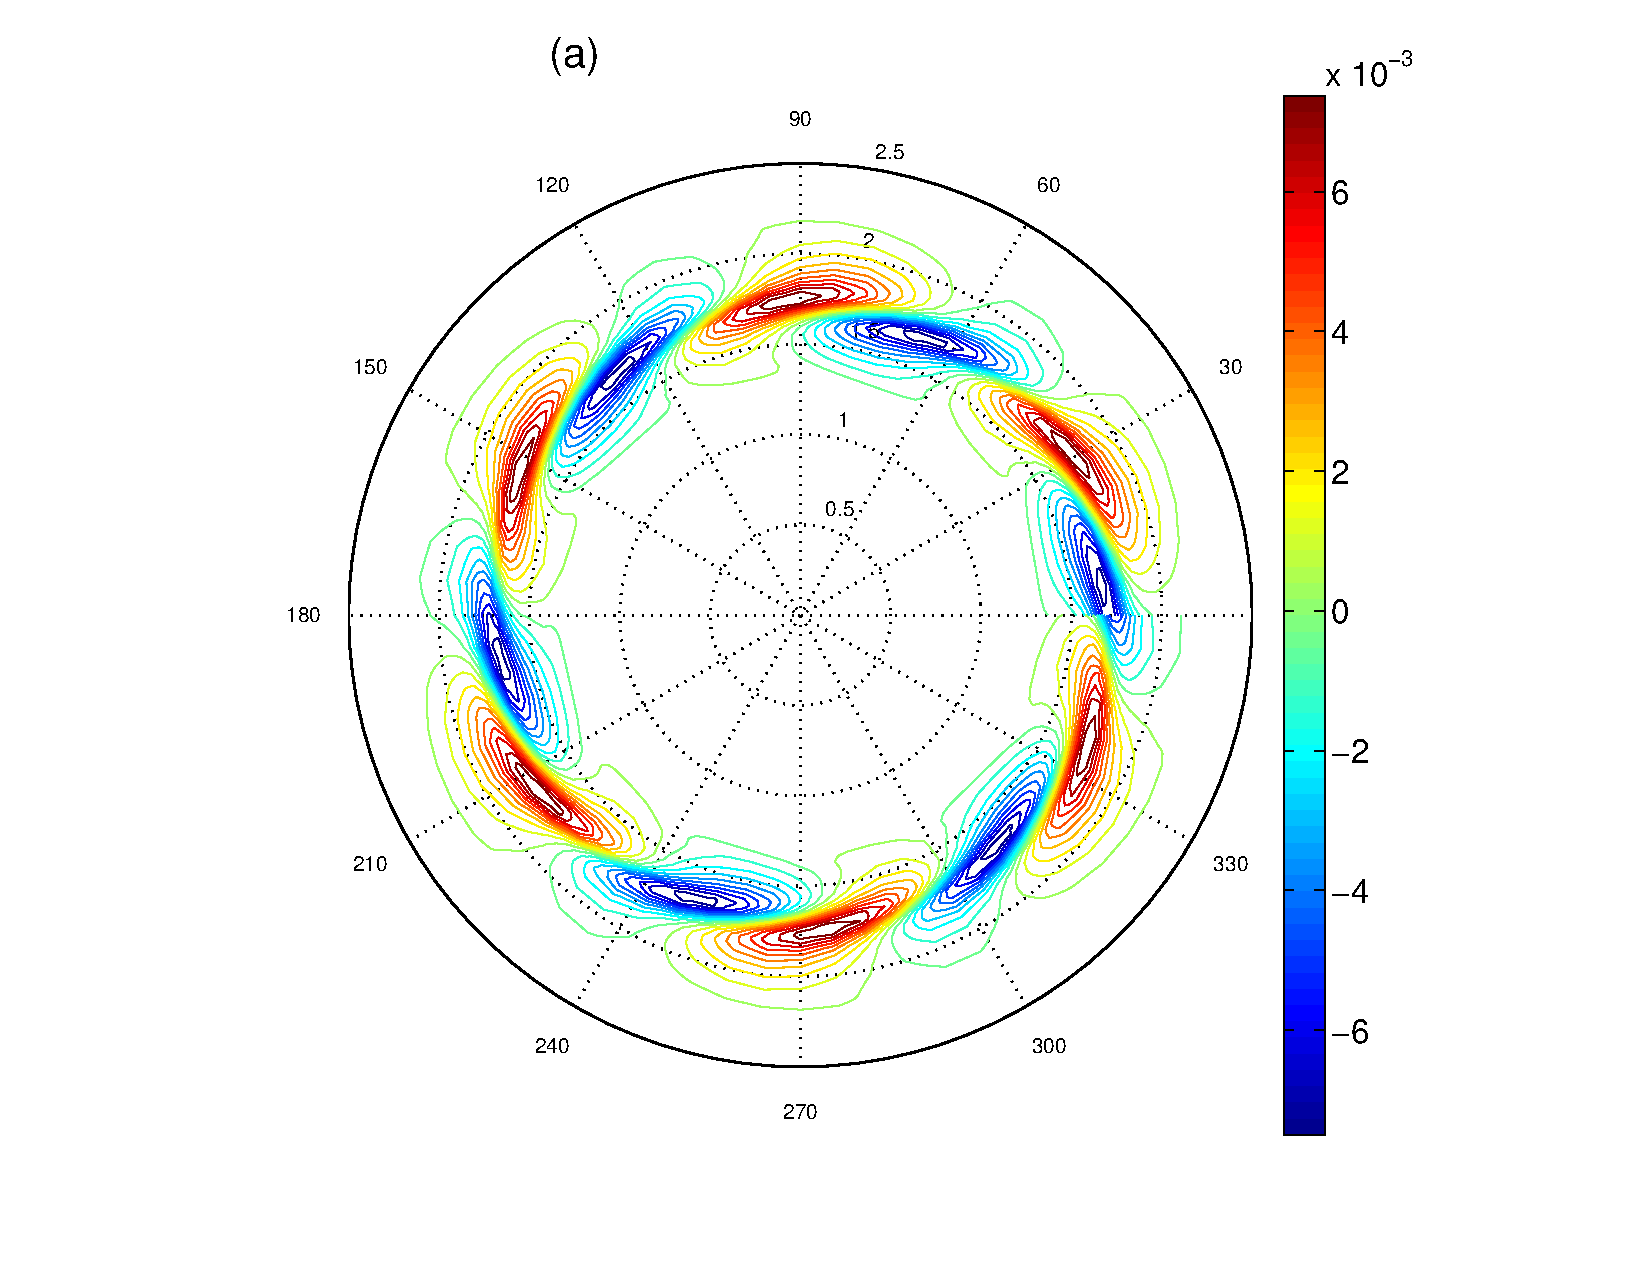
\includegraphics[height = 6cm, keepaspectratio]{./figures/Pictures/pot_ele}}&
{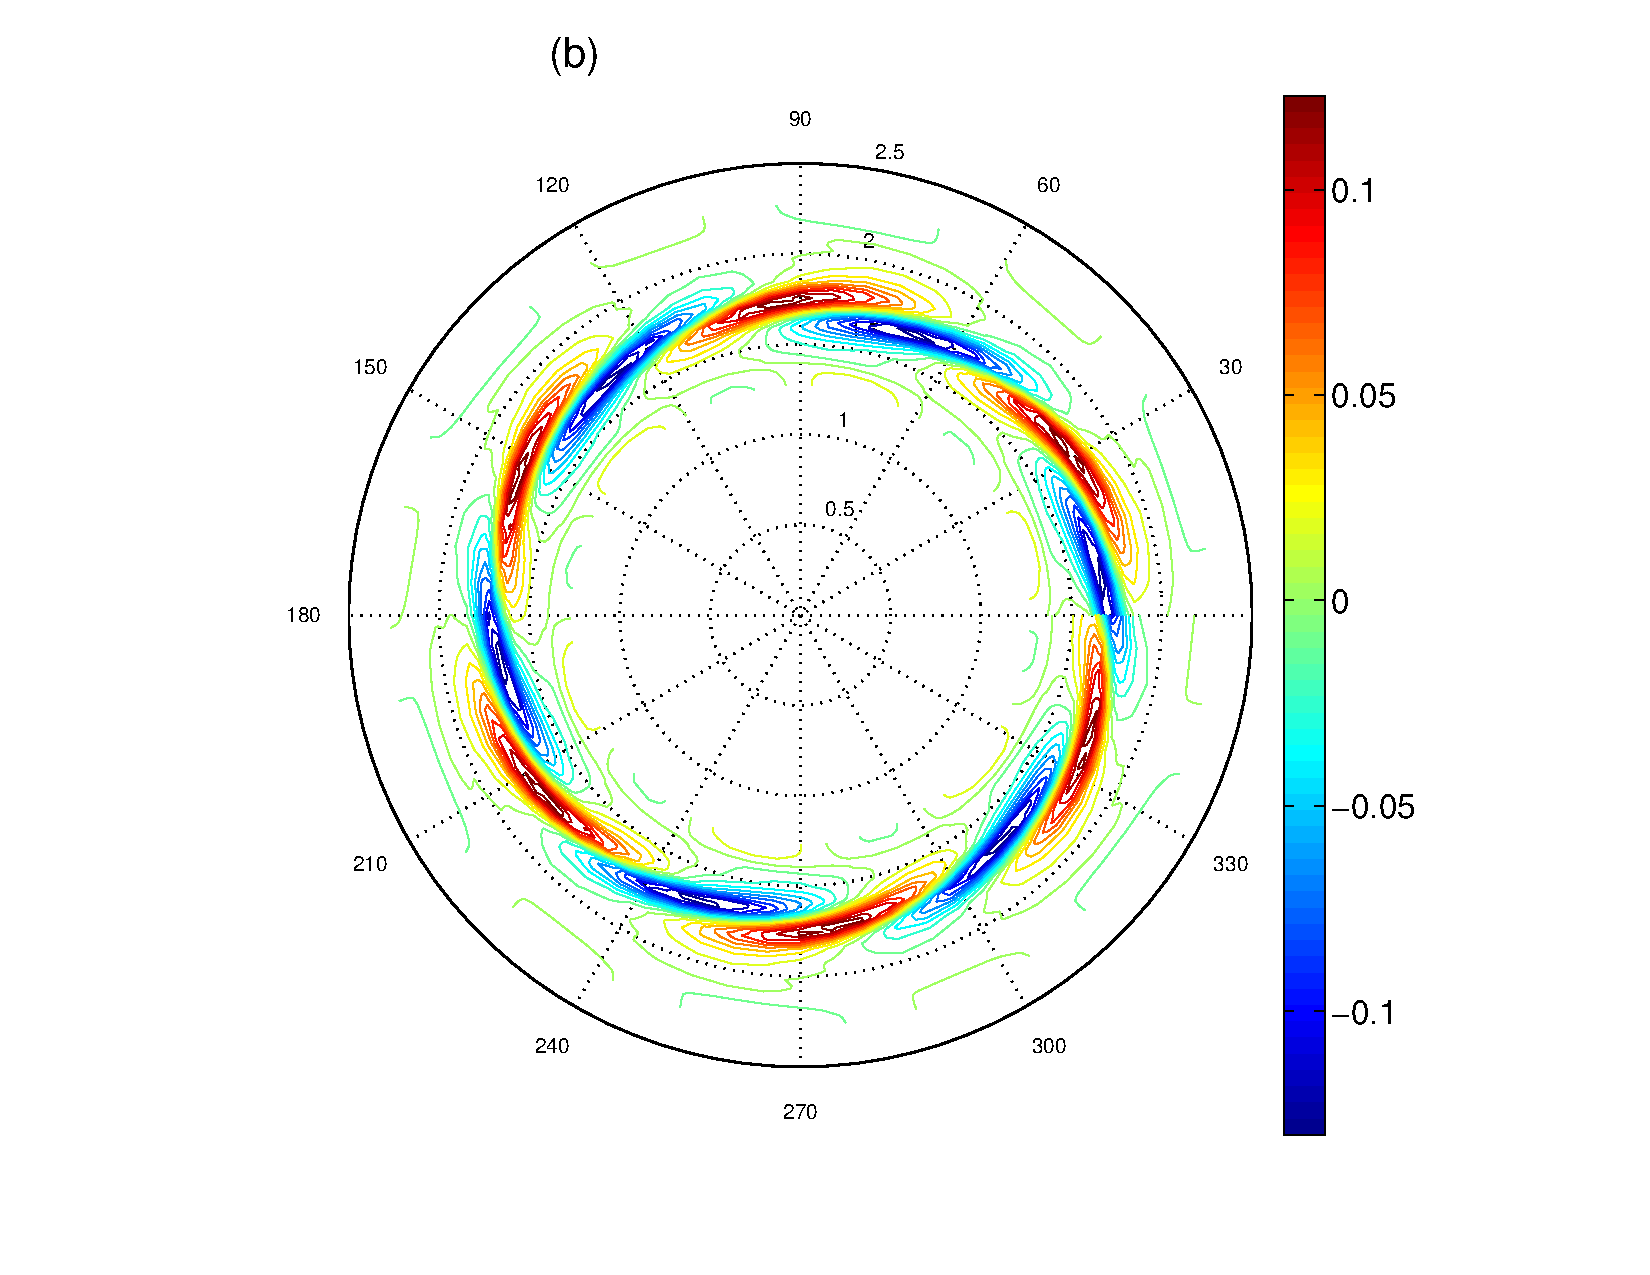
\includegraphics[height = 6cm, keepaspectratio]{./figures/Pictures/charge_dens}}\\
{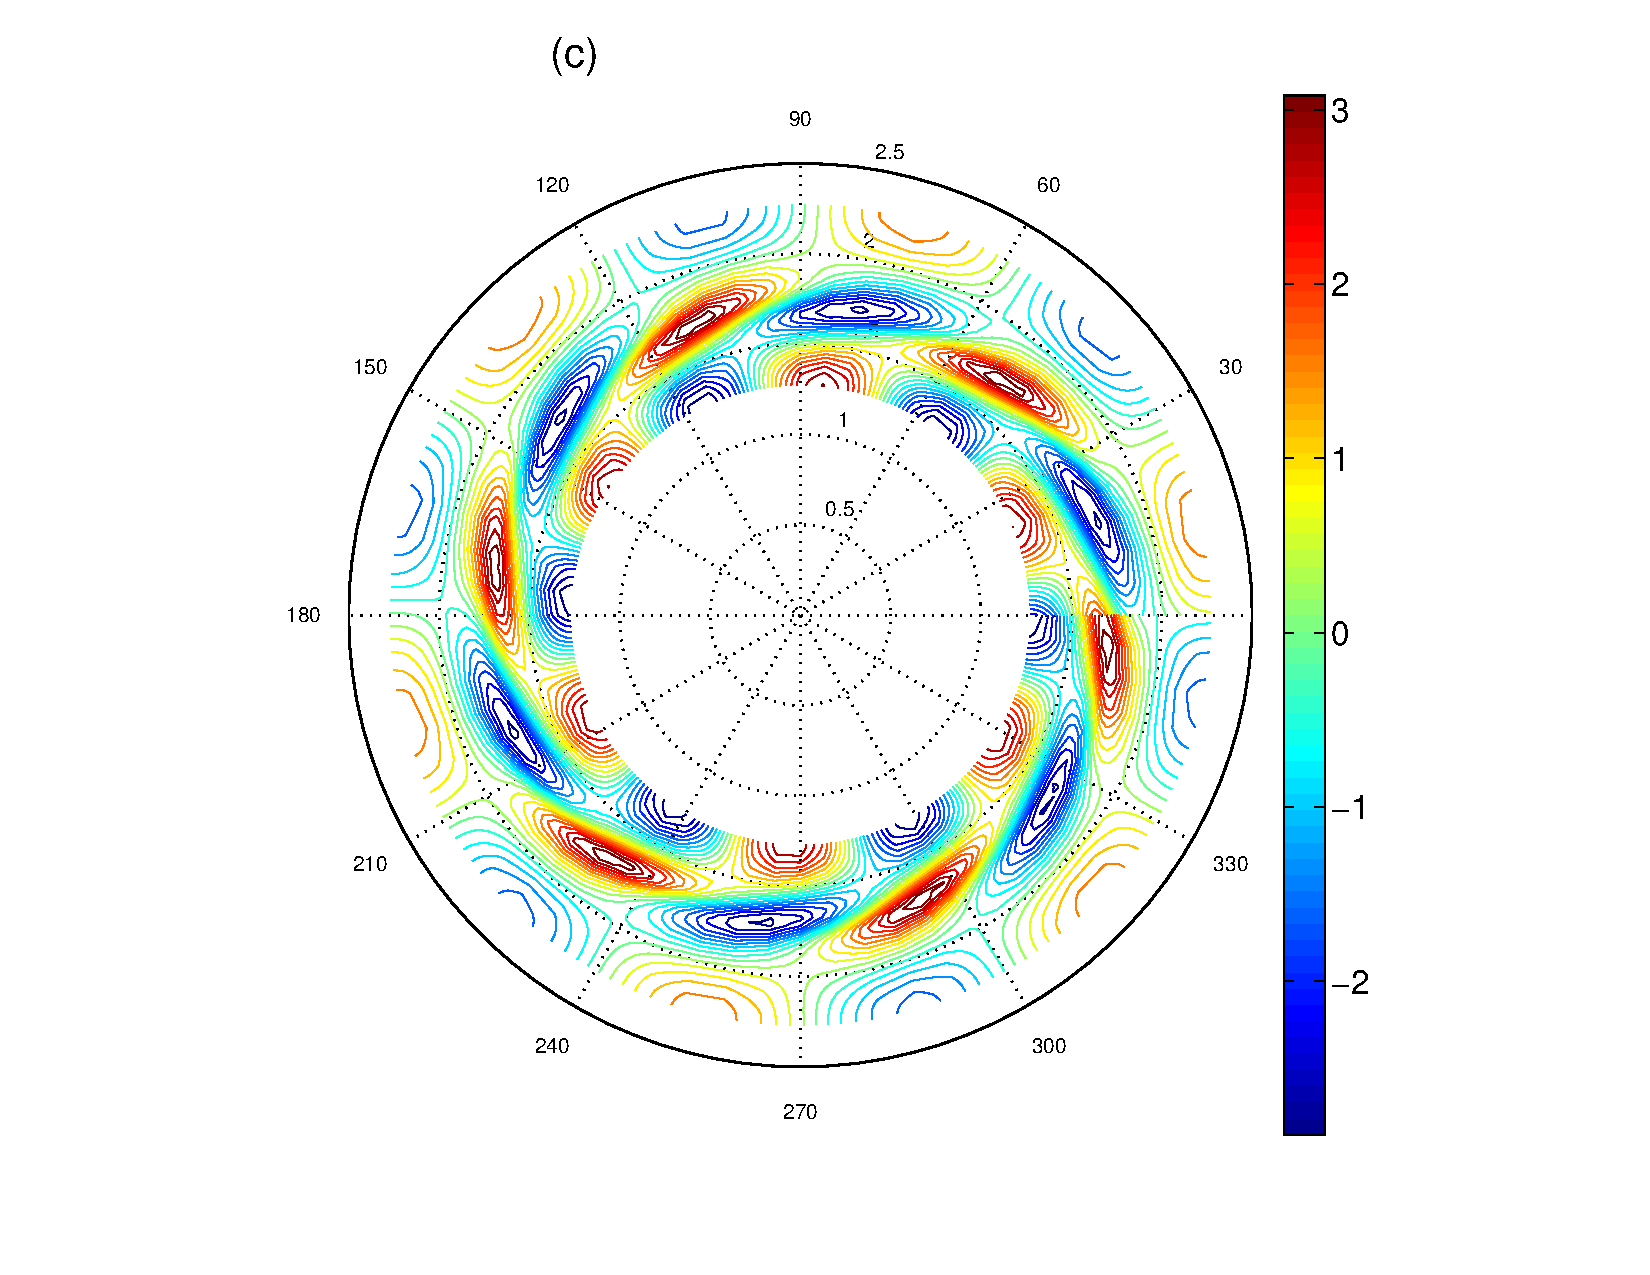
\includegraphics[height = 6cm, keepaspectratio]{./figures/Pictures/vorticity}}&
{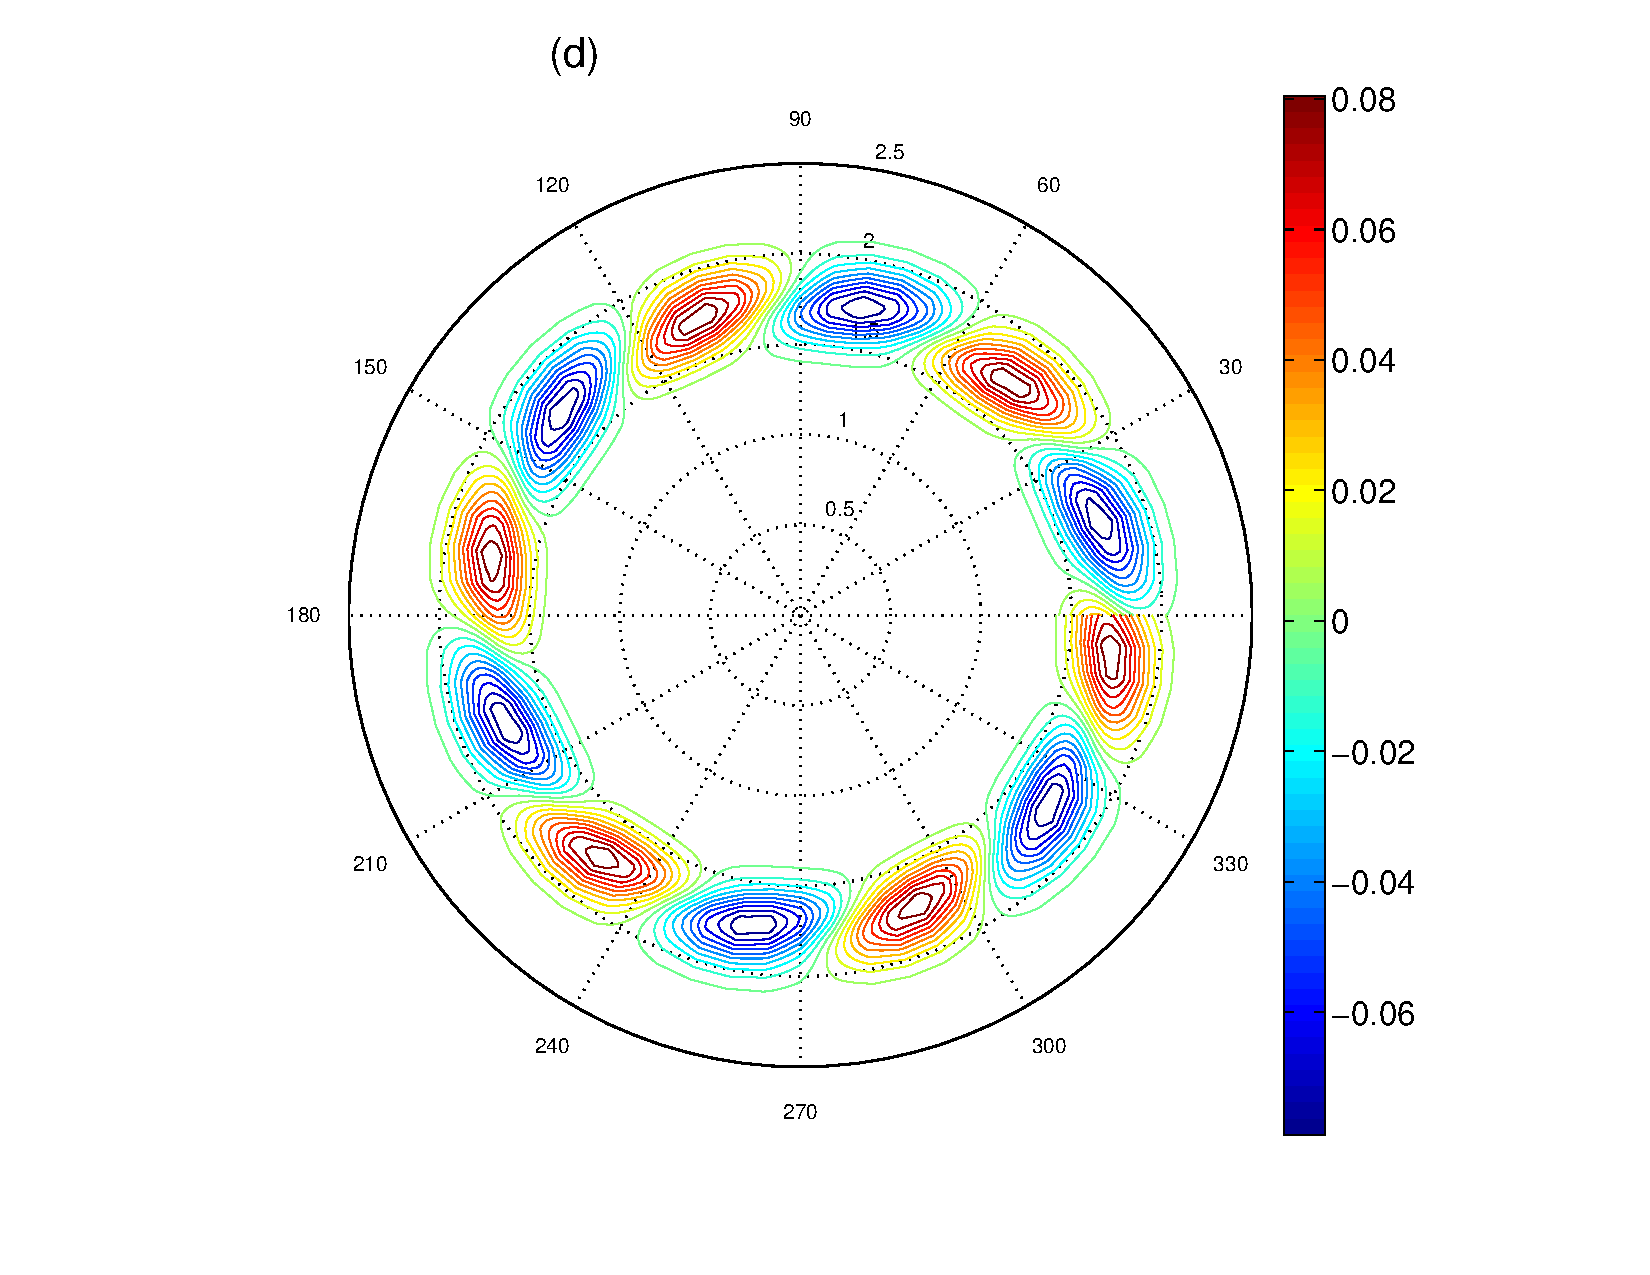
\includegraphics[height = 6cm, keepaspectratio]{./figures/Pictures/stream_fun}}\\
\end{tabular}
\caption{Numerical results of the perturbation of the four physical quantities for $\mathcal{R}_c<\mathcal{R}<\mathcal{R}_{c_2}$: the 2D electric potential $\psi_2$ in (a), the charge distribution $q$ in (b), the vorticity $\omega$ in (c) and the streamfunction $\phi$ in (d).   }
\label{phy_quan_rot_waves}
\end{figure}

Using the matrix-free numerical bifurcation method, the secondary bifurcation is identified at $\mathcal{R}_{c_2} = 636 = 1.11\mathcal{R}_c$. This is also a Neimark-Sacker bifurcation corresponding to the transition from the rotating wave flow. Thus we can conclude that for $ 572 < \mathcal{R} < 636$ the rotating wave flow is asymptotically stable and unstable for $\mathcal{R} > \mathcal{R}_{c_2} = 636$. To validate these results, we have simulated the solutions corresponding to the rotating waves with some perturbations for $\mathcal{R} = 632 < \mathcal{R}_{c_2}$ at which the solution is stable and for $\mathcal{R} = 640 > \mathcal{R}_{c_2}$ where the equilibrium solution becomes unstable.
We observe in Figure~\ref{phy_quan_rot_waves} that in the regime where the rotating waves are stable, the flow velocity and the electric field are periodic and there is no change in magnitude.

In the regime where the rotating waves are unstable, the perturbation grows and both the flow velocity and the electric fields oscillate. An illustration of the perturbation of the streamfunction $\phi$ is shown in Figure~\ref{snap} at a different time of the simulation as compared to that of Figure~\ref{phy_quan_rot_waves}. Figure~\ref{proj_phase} further exemplifies this oscillation by showing a time-series after the secondary transition. This time-series also validates that a single frequency periodic limit cycle at the secondary transition evolves into waves that vacillate with an increasing maximum amplitude beyond this transition point. The phase space plot of both the rotating waves and amplitude vacillating waves are contrasted in Figure~\ref{proj_phase}.

\begin{figure}[t]
\centering
\subfigure[][]{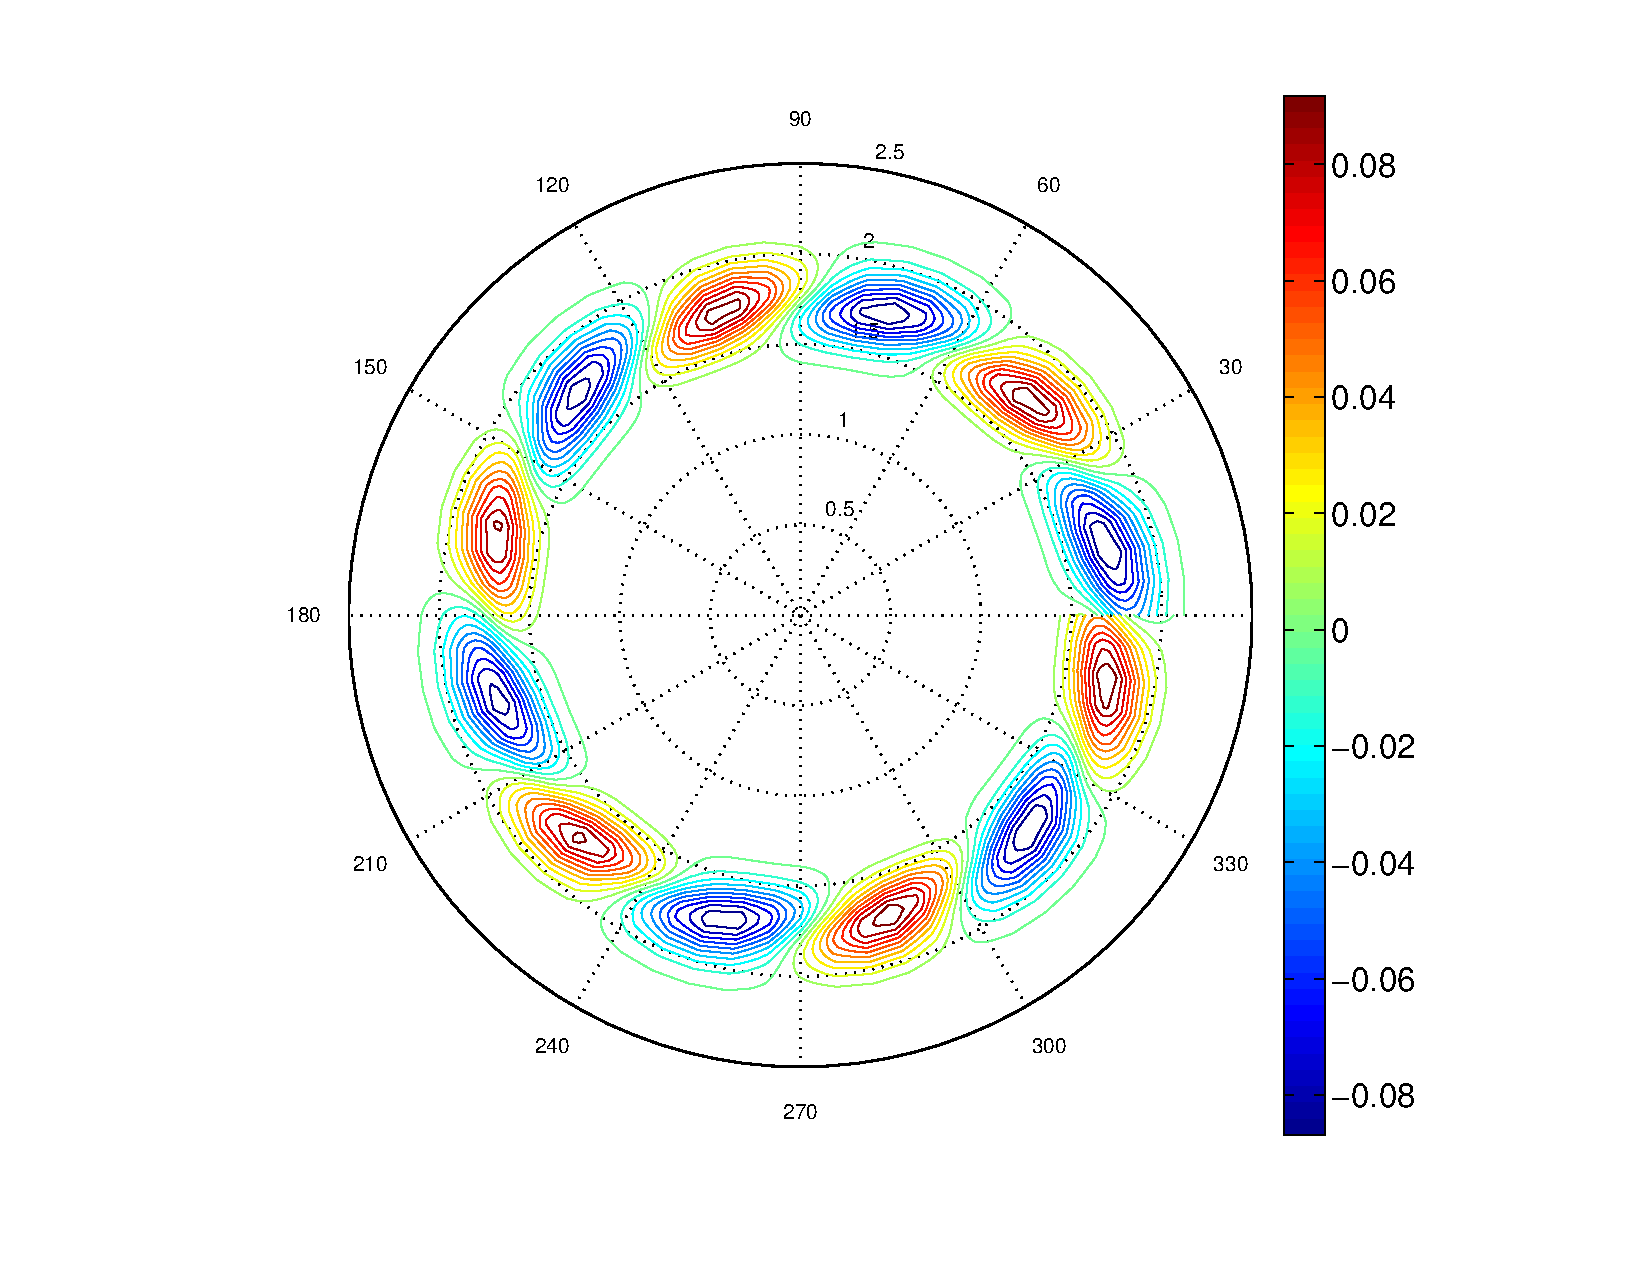
\includegraphics[width = 0.45\textwidth]{./figures/Pictures/snapshot_amp_vac1}}
\hspace{8pt}
\subfigure[][]{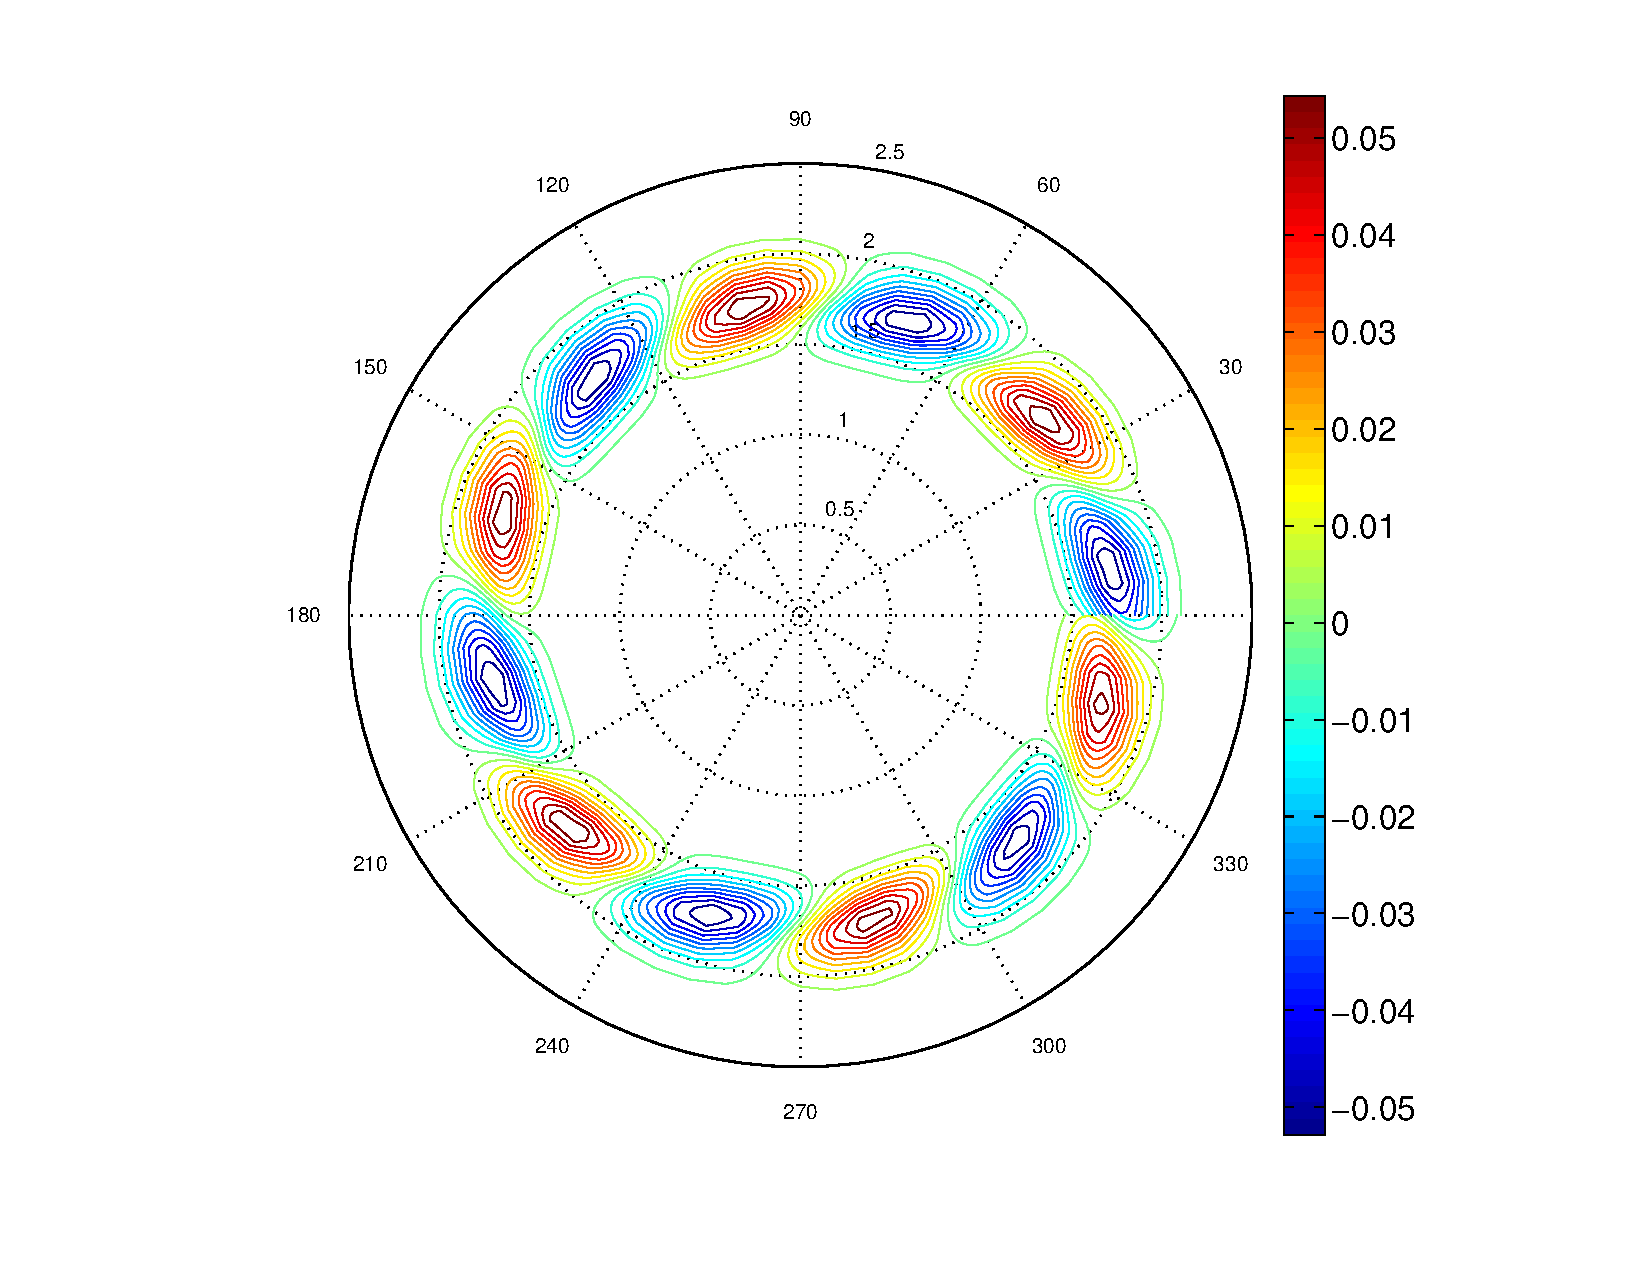
\includegraphics[width = 0.45\textwidth]{./figures/Pictures/snapshot_amp_vac2}}
\hspace{8pt}
\subfigure[][]{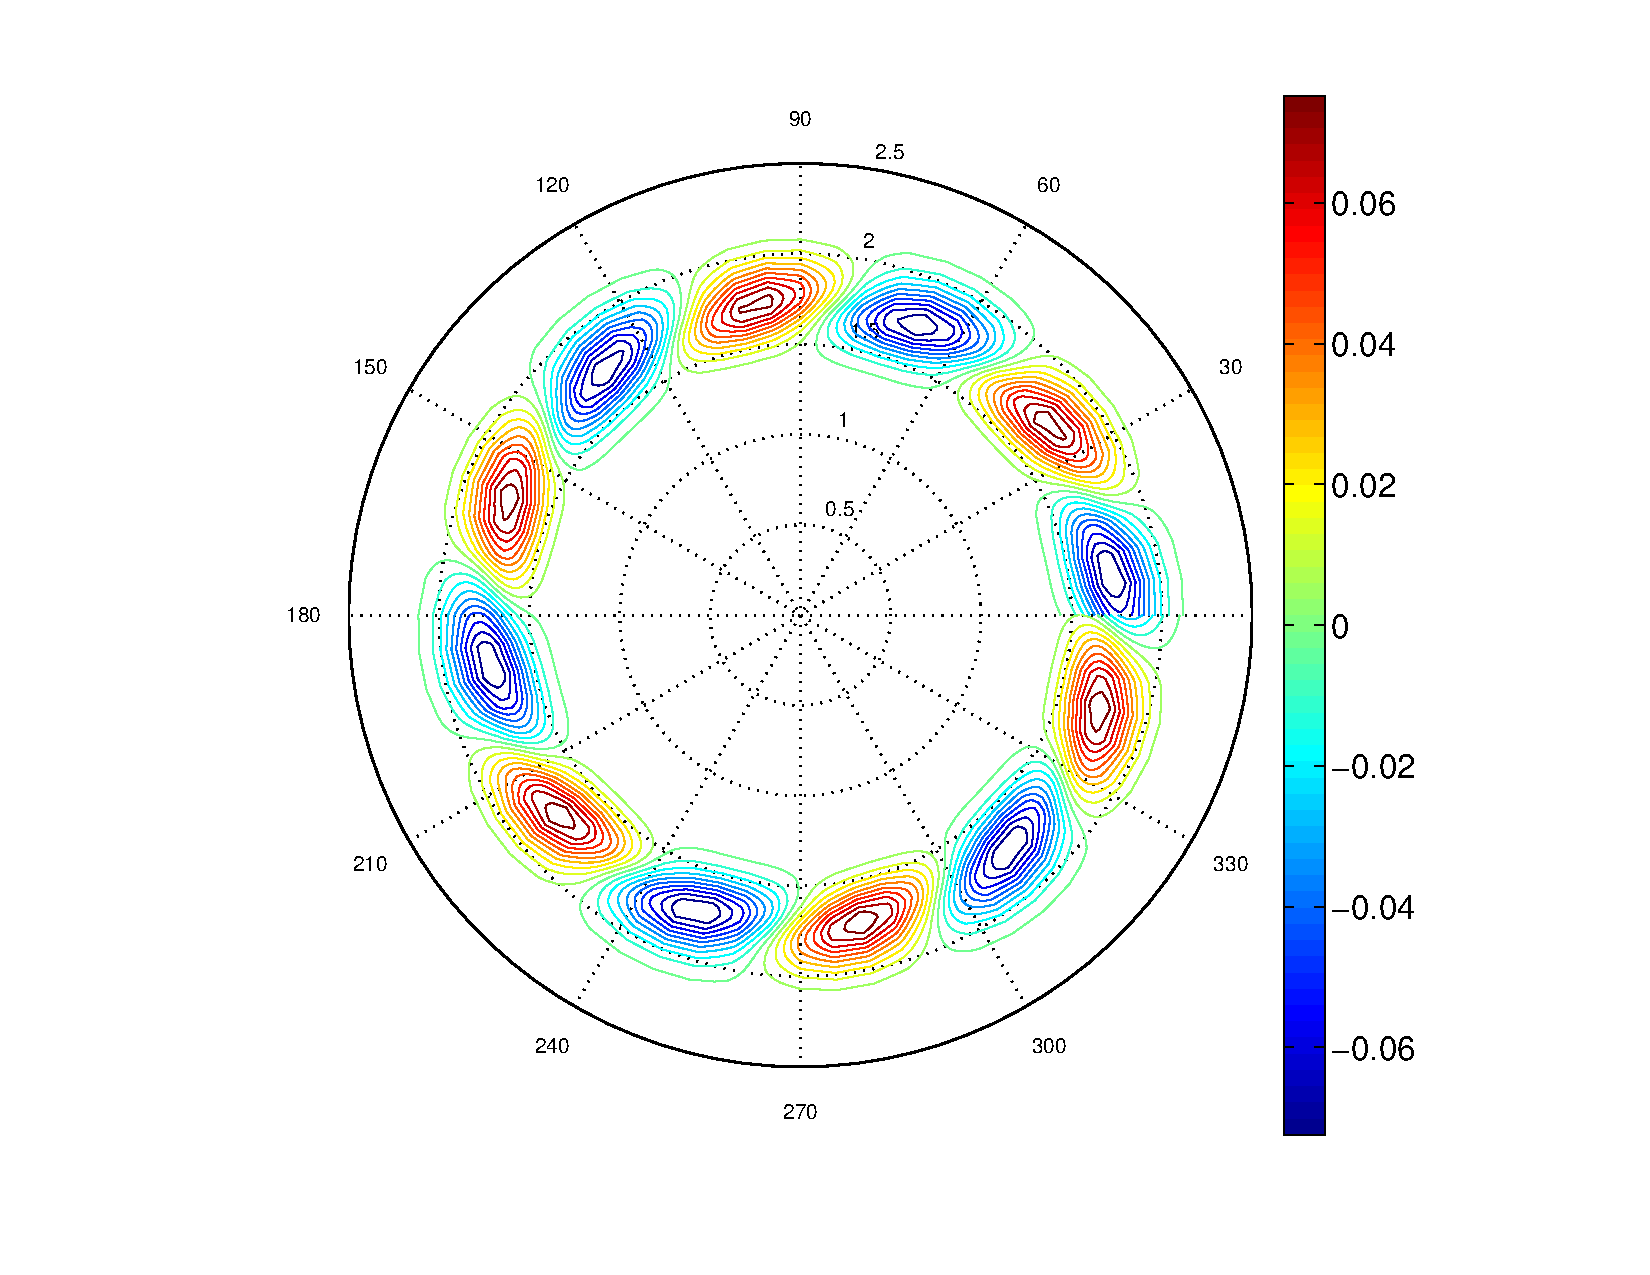
\includegraphics[width = 0.45\textwidth]{./figures/Pictures/snapshot_amp_vac3}}
\hspace{8pt}
\subfigure[][]{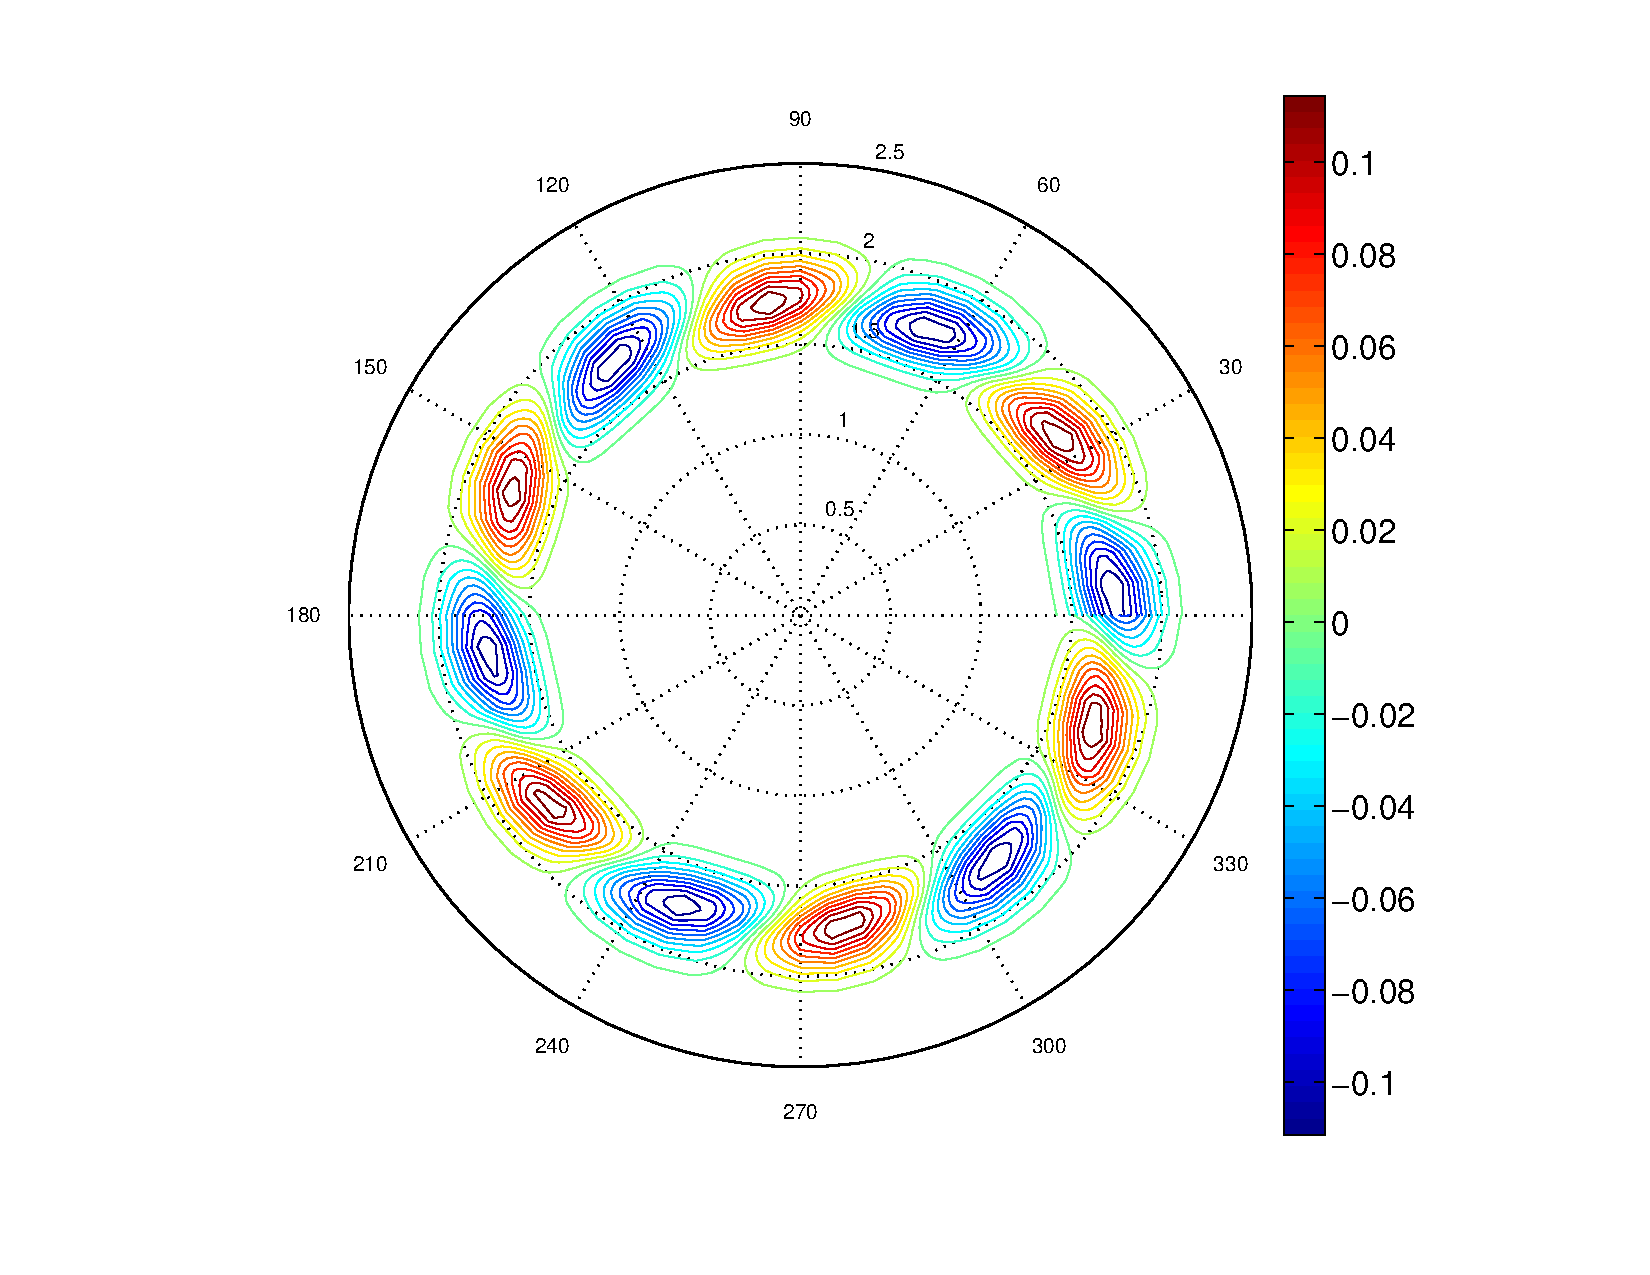
\includegraphics[width = 0.45\textwidth]{./figures/Pictures/snapshot_amp_vac4}}
\caption{Snapshots of a simulation of the perturbation of the streamfunction $\phi$ from the base state at different times within a period of the vacillation at $\mathcal{R} = 640$. The amplitude of the wave oscillates as indicated by the color bar. }
\label{snap}
\end{figure}


\begin{figure}[t]
\centerline{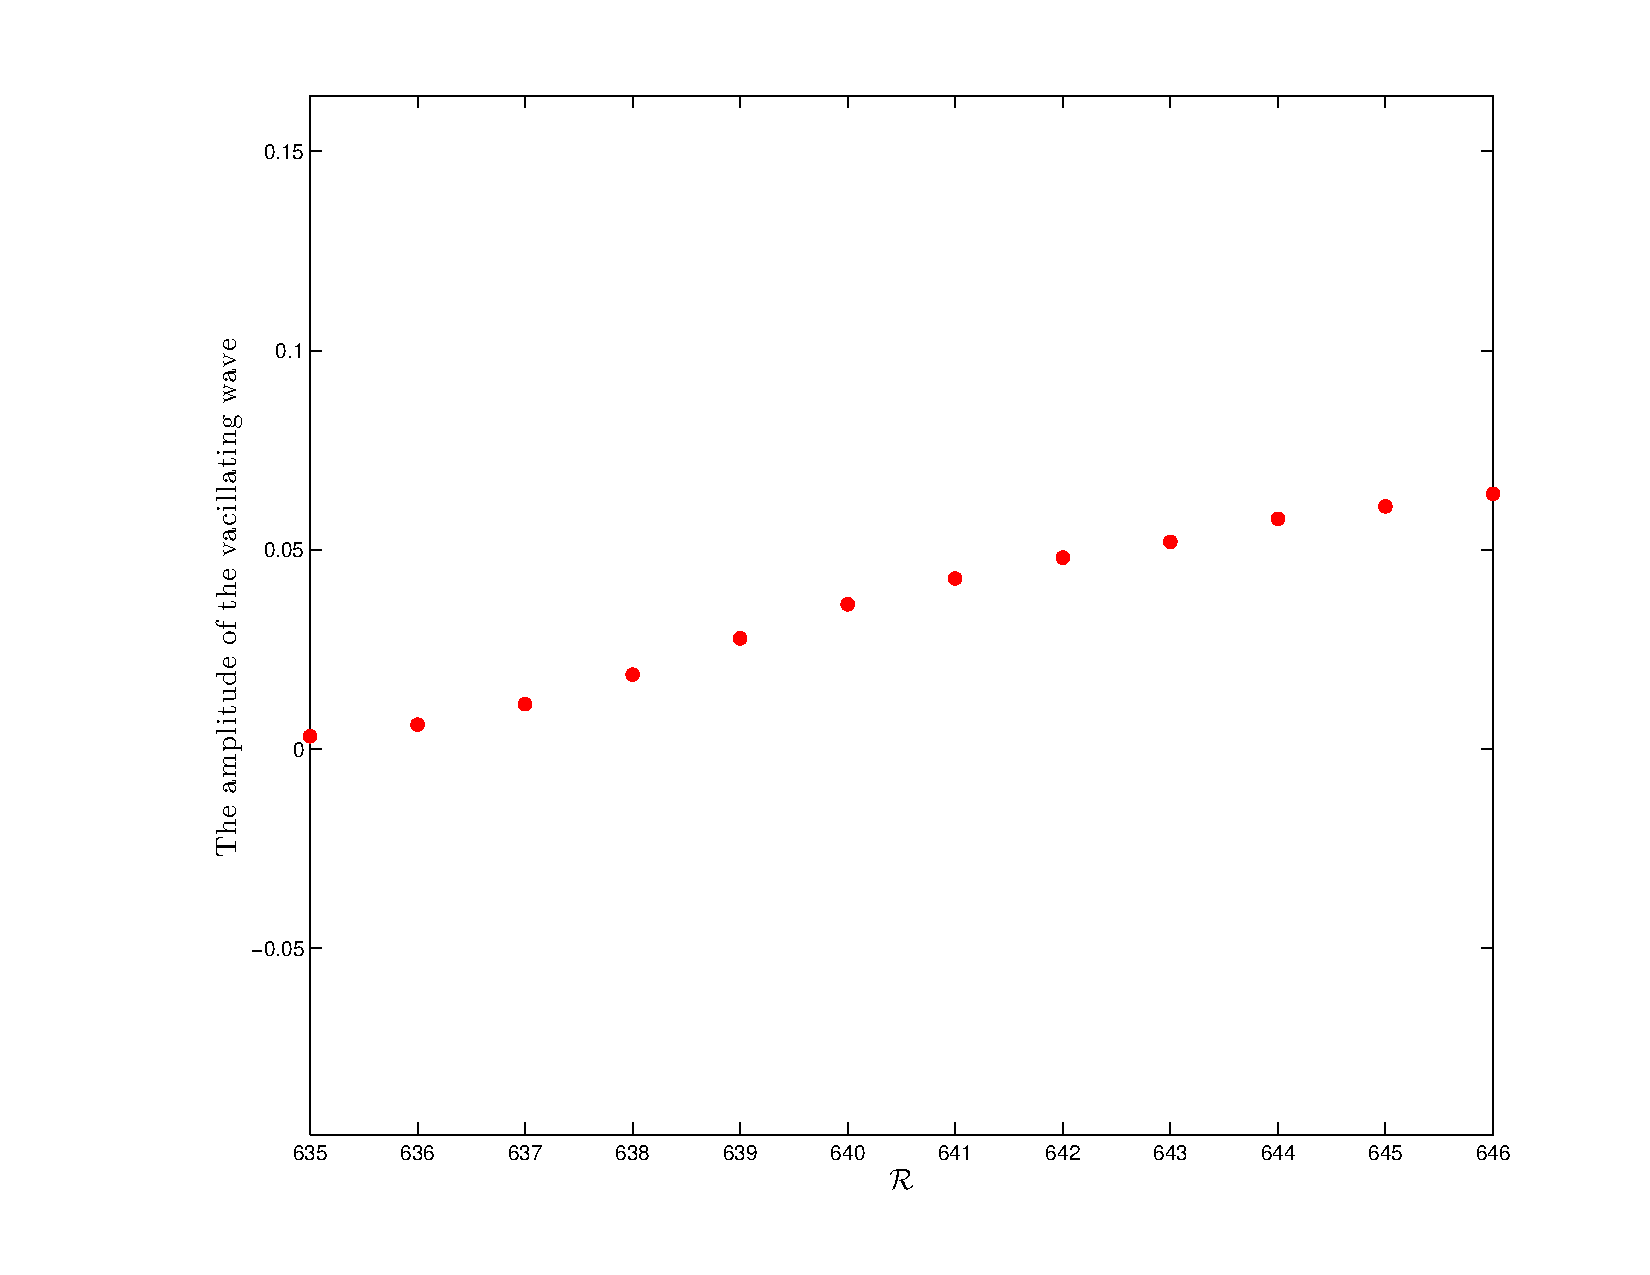
\includegraphics[width = .9\textwidth]{./figures/Pictures/Amplitude_vacillating}}
\caption{Time-series of the amplitude of the vacillating wave for Rayleigh number $\mathcal{R}$ beyond the secondary transition.}
\label{amp_vac}
\end{figure}

This bifurcation cannot be identified  as supercritical or subcritical from the techniques we have used. However, we have simulated the solution corresponding to the rotating waves state with a random perturbation of magnitude $10^{-2}$
for $t = 30$ (60000 time steps) in the unstable region, $636 \le \mathcal{R} \le 646$. The amplitude of vacillation for the vacillating waves is obtained by computing the difference between the maximum and the minimum envelope value within a given cycle. Figure~\ref{amp_vac} shows that the amplitude of the vacillation is found to grow monotonically from zero with zero corresponding to the rotating waves. This result shows evidence that the bifurcation is likely supercritical. To confirm this, we would need to compute the normal form coefficient of the map, which we choose not to do due to the complexity of its computation.

\begin{figure}[t]
\centering
\subfigure[][]{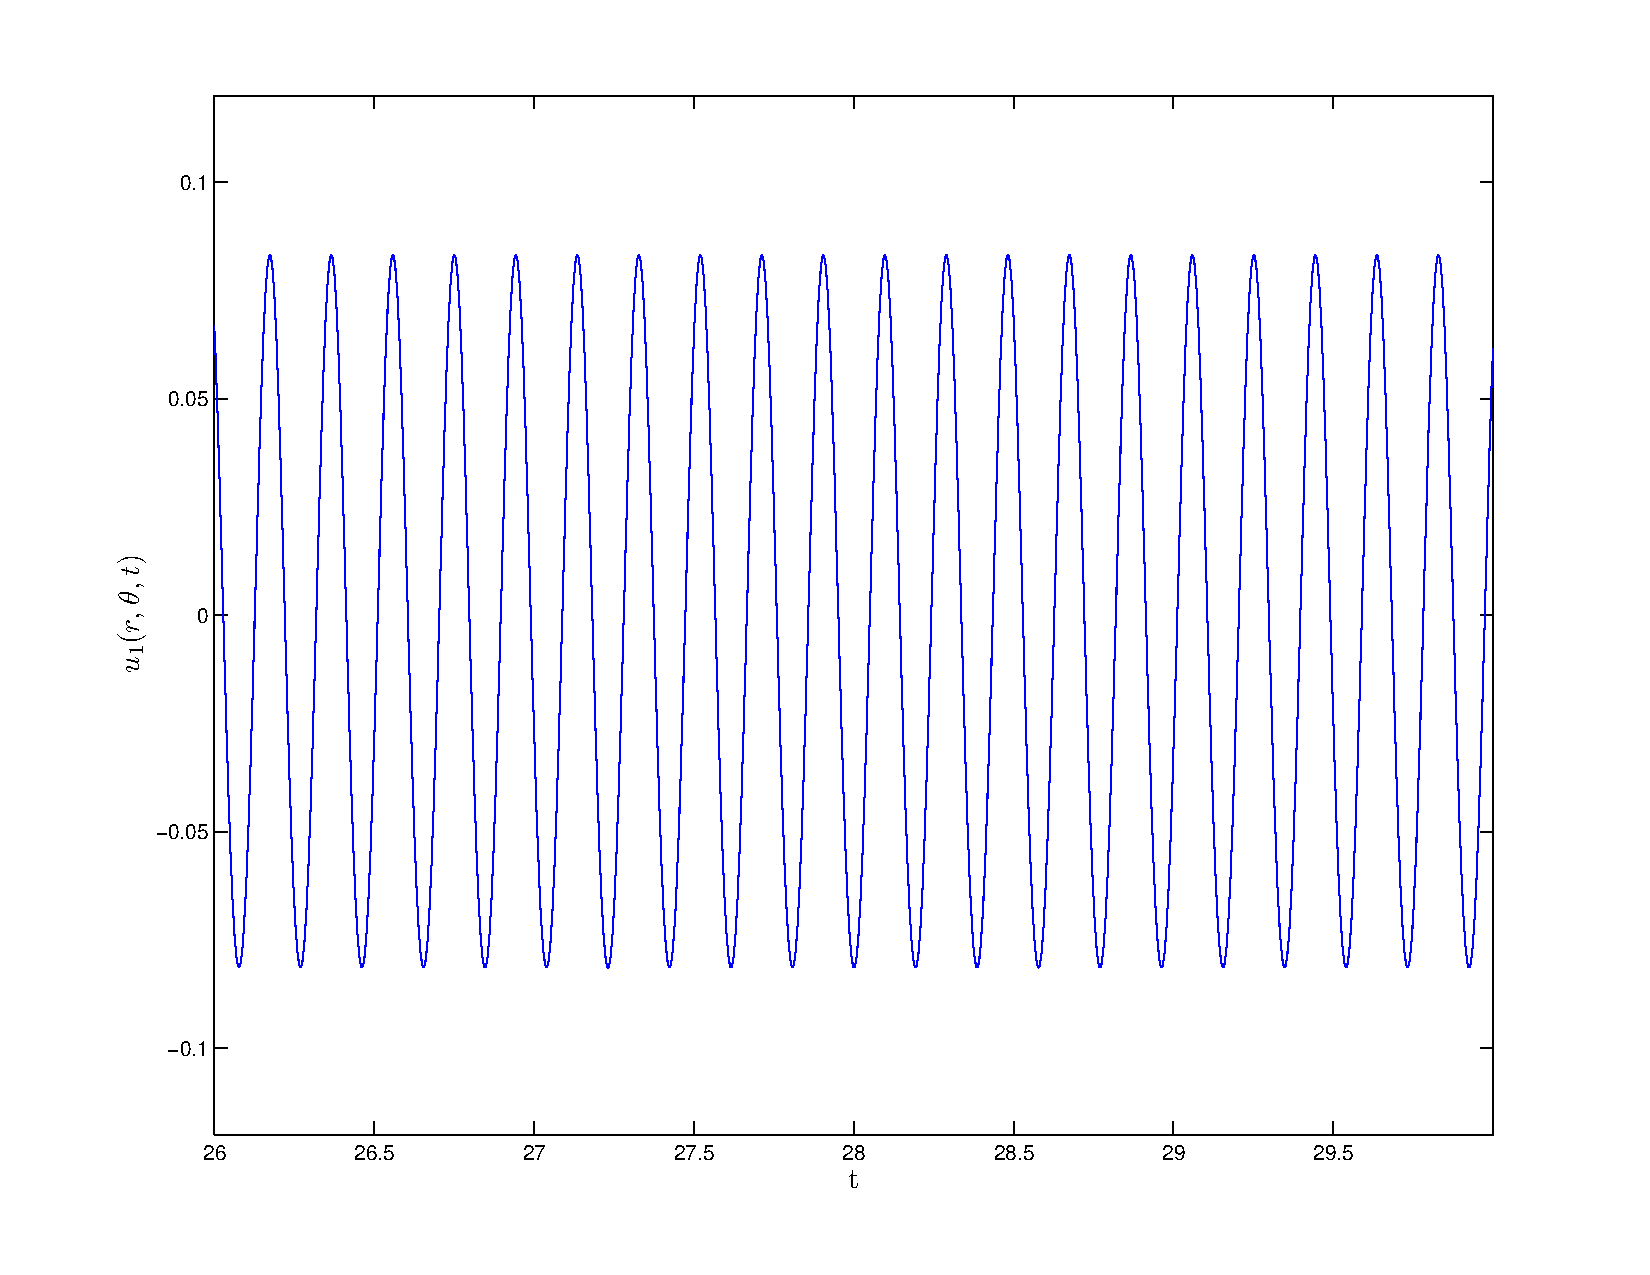
\includegraphics[width = 0.45\textwidth]{./figures/Pictures/time_phase_Ra_632_640_1}}
\hspace{8pt}
\subfigure[][]{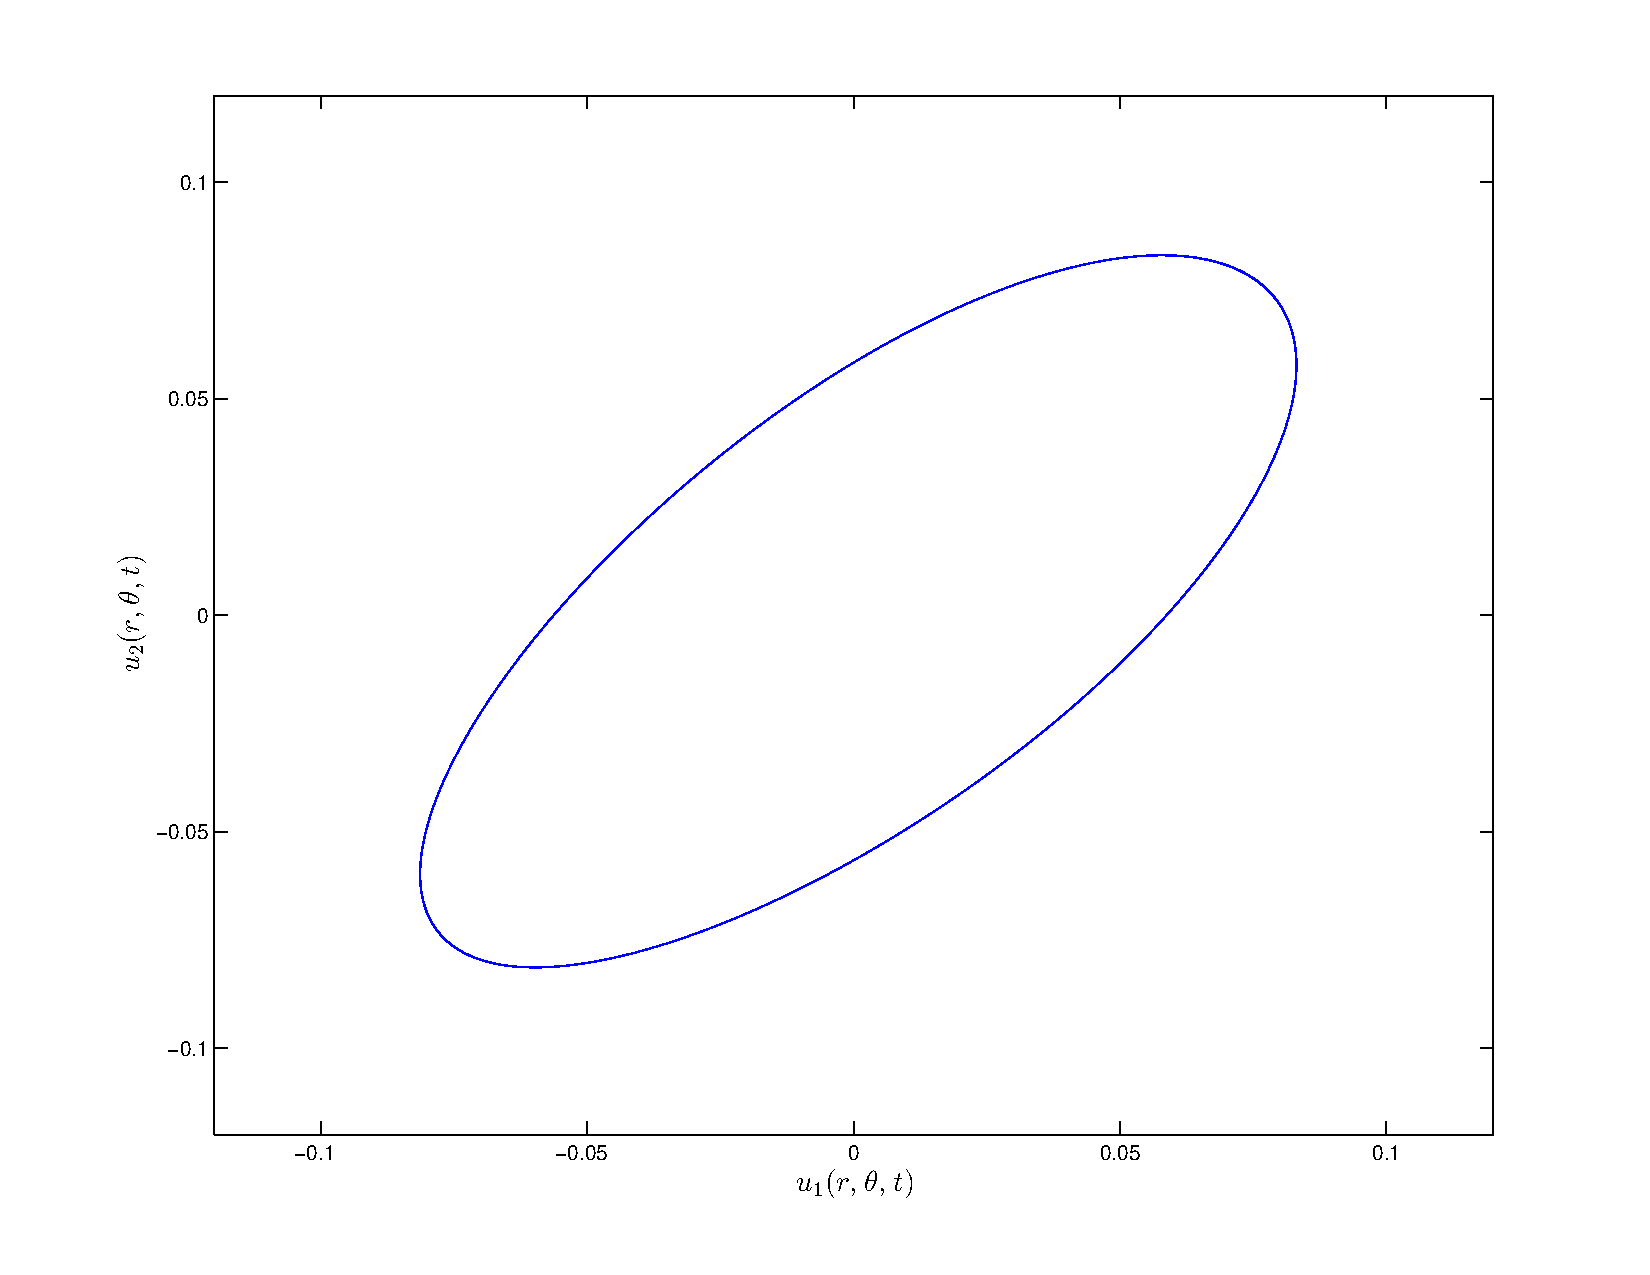
\includegraphics[width = 0.45\textwidth]{./figures/Pictures/time_phase_Ra_632_640_2}}
\hspace{8pt}
\subfigure[][]{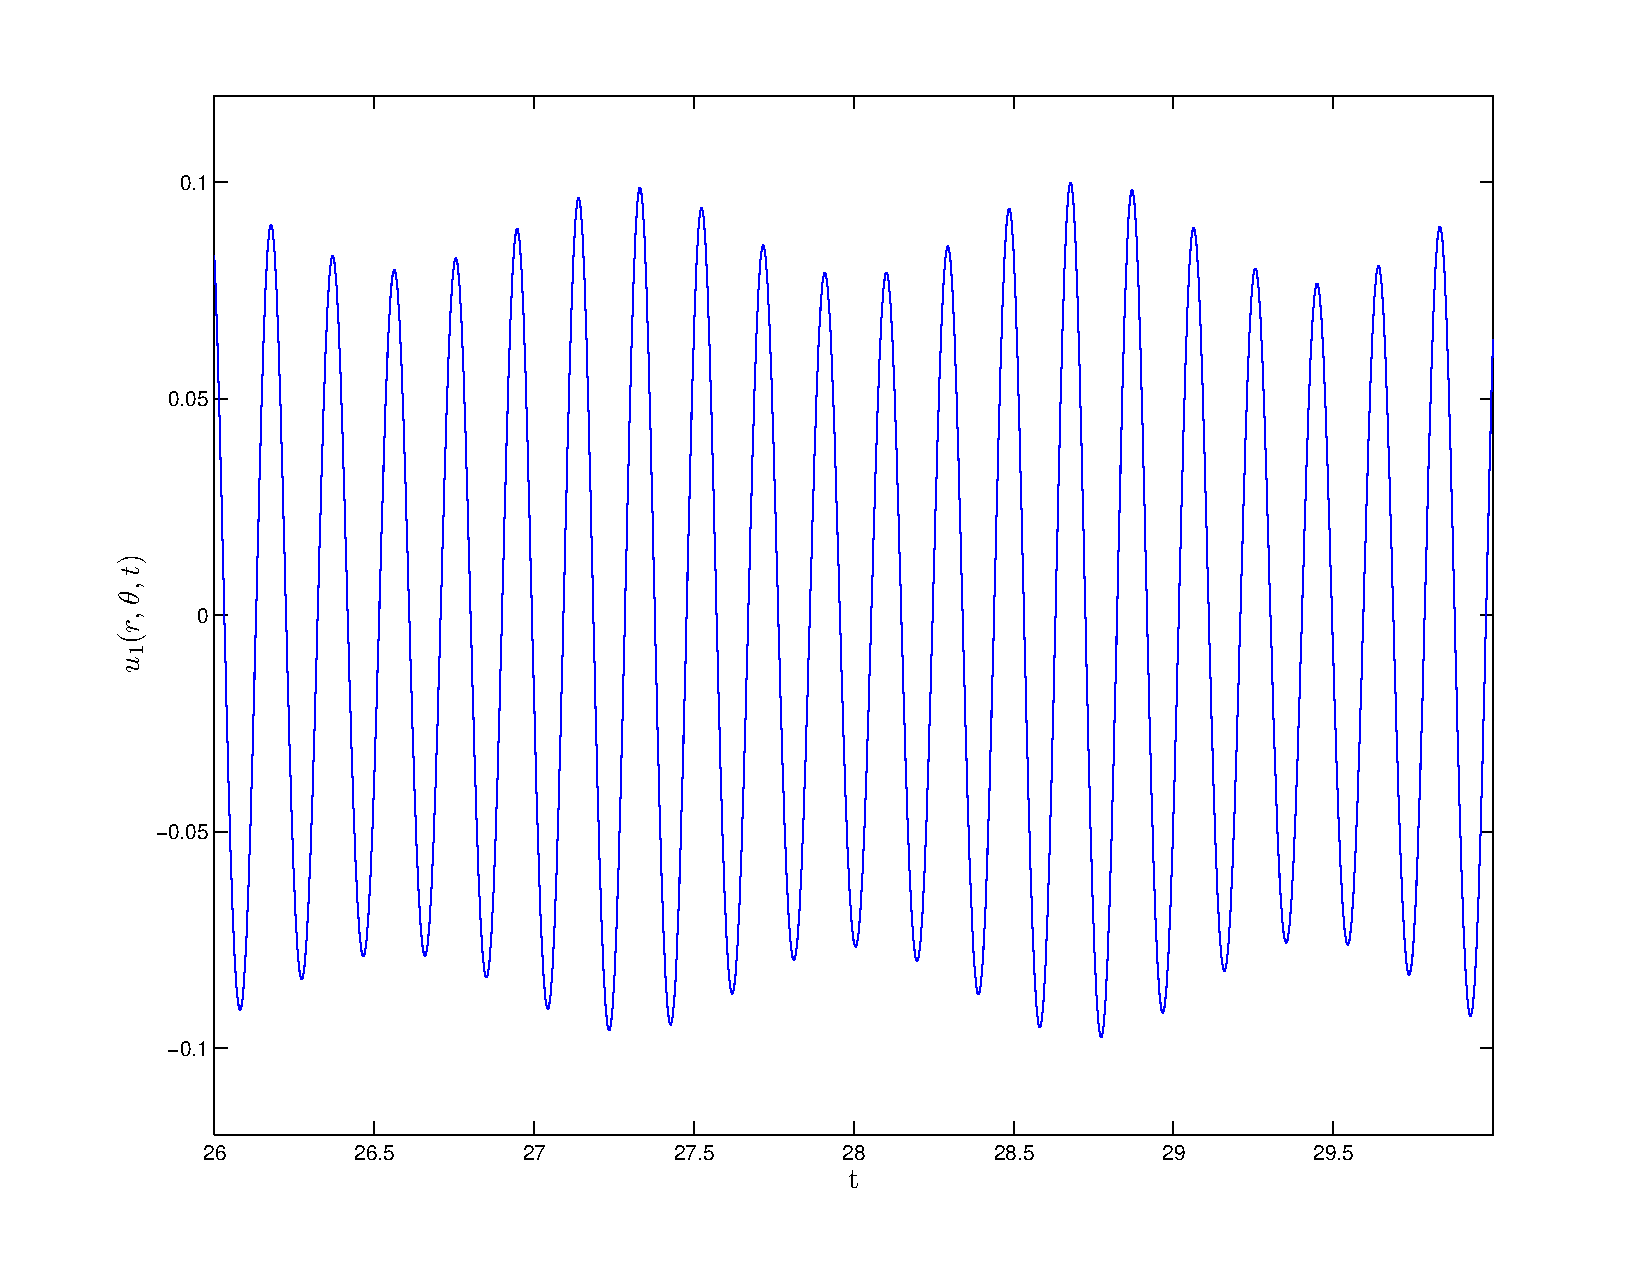
\includegraphics[width = 0.45\textwidth]{./figures/Pictures/time_phase_Ra_632_640_3}}
\hspace{8pt}
\subfigure[][]{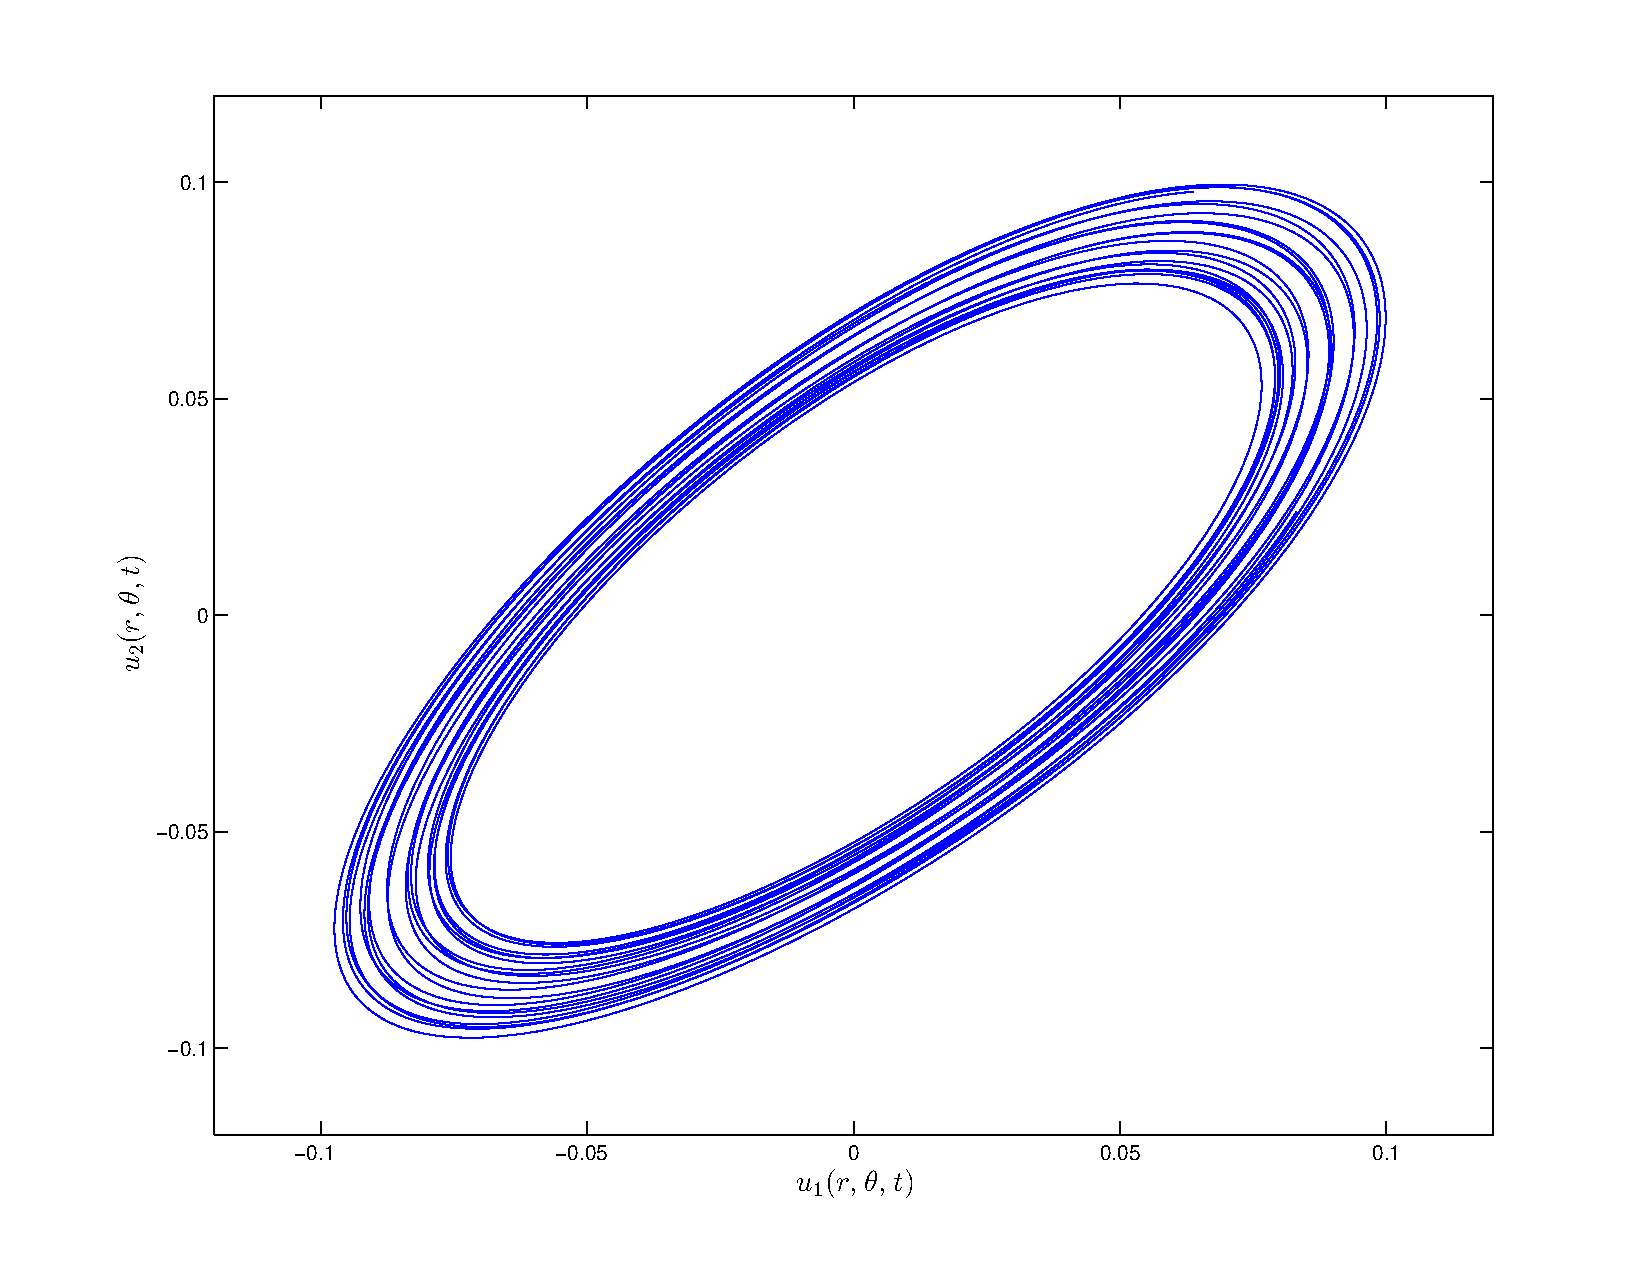
\includegraphics[width = 0.45\textwidth]{./figures/Pictures/time_phase_Ra_632_640_4}}
\caption{Comparison of the phase portraits of projections of the two solutions at $\mathcal{R} = 632 $ in (a), (b) and at $\mathcal{R} = 640$ in (c), (d).}
\label{proj_phase}
\end{figure}

To summarize, we have identified two Neimark-Sacker bifurcations at $\mathcal{R}_c = 572$ and $\mathcal{R}_{c_2} = 636$.
At the bifurcation point $\mathcal{R}= 572$, there is a change in the stability of the fixed point from stable to unstable, with a stable limit cycle appearing at the bifurcation point. Therefore, the primary bifurcation is a supercritical Neimark-Sacker corresponding to a supercritical Hopf bifurcation in the continuous dynamical system.
For a more detailed explanation of the Neimark-Sacker bifurcation, the reader is referred to~\cite{Kuznet}. Tracing the solution curve corresponding to the rotating waves state while decreasing the Rayleigh number, emphasizes that the bifurcation is supercritical.
%The primary bifurcation from an axisymetric state to a rotating waves state is a Neimark-Sacker bifurcation. This bifurcation is a supercritical Neimark-Sacker since a transition in the stability of the fixed point occurs from stable to unstable and a stable limit cycle appears at the bifurcation point. For a more detailed explanation the reader is referred to \cite{Kuznet} to learn more about the bifurcations of a map.

The secondary bifurcation is also a Neimark-Sacker bifurcation corresponding to the transition between the rotating waves state to the amplitude vacillating wave states. The type of this secondary bifurcation cannot be identified as supercritical or subcritical from the techniques used. However, evidence suggests that the bifurcation is more likely to be a supercritical and to confirm its type, we need to compute the normal form coefficient of the map.

\section{Discussion}
Previous scholars have investigated the primary transition of the flow using different techniques; experimentally~\cite{BAEWIS,AEWSDaDe}, analytically~\cite{EDCTAFUCF,linearstability}, and using direct numerical simulation~\cite{PeiChunTsain,DNSSAE,LSSE-PeDa}, also known as numerical experimentation. In this thesis, we focus on the comparison of our results, using the matrix-free numerical bifurcation method, to previous results obtained, that showed successive transitions of the flow as the Rayleigh number is gradually increased. The flow undergoes transitions from axisymmetric to rotating wave to amplitude vacillating waves to another rotating wave involving a different mode, and eventually the flow becomes chaotic.  The primary transition was shown to be a supercritical Hopf bifurcation for various parameters of the system.

In the previous section, the primary transition was shown to occur at the critical Rayleigh number, $\mathrm{R}_c = 572$, with a critical mode, $ m_c = 6$, for the parameters in Table~\ref{table_para}. These results are in agreement with those obtained in~\cite{PeiChunTsain}.
The secondary transition to the amplitude vacillating waves was identified at $\mathrm{R}_{c_2} = 636$. This result is not comparable to other literature due to the difference choice of Reynolds number. To confirm the secondary transition, we simulated the periodic solution obtained from the continuation method, with a random perturbation of magnitude $10^{-2}$, for $\mathcal{R} = 632$ and $\mathcal{R} = 640$ over relatively long time. For $\mathcal{R} = 632$, the solution converged to the rotating wave flow, and for $\mathcal{R} = 640$, the solution converged to the amplitude vacillating waves.
%This simulation provides further evidence that there is a transition from the rotating waves state to the amplitude vacillating wave state.












%%
%\section{Transition from steady to periodic}
%At this point, we have implemented a matrix free continuation method based on the natural parametrization using a secant extrapolation as a predictor step and a Newton-Krylov nonlinear solver as a corrector step to detect and compute two type of equilibria (the homogeneous steady state and the periodic orbit) for a dynamical system.
%This methods was applied on the annular sheared electroconvection discussed in chapter 2. The electroconvection model involves four different dimensionless parameters; the Rayleigh number $\mathcal{R}$ the main control parameter of interest, and  three other parameters we fixed the Prandlt number $\mathcal{P} = 75.8$, the aspect ratio $\alpha = 0.56$ and the Reynolds $Re = .249$. We traced the solution curve by varying the Rayleigh number $\mathcal{R}$ where we computed the equilibria solution for the respective Rayleigh number. Upon obtaining the equilibria solution, a linear stability analysis has been conducted to investigate the stability of these equilibria by solving the eigenvalue problem. The results are presented in Figure~\ref{bif_diag}. We compose the figure by tracing the zero solution of the perturbation equations of the model corresponding to the axisymmetric solution and we found the critical Rayleigh number $R_c = 572$ at which the transition to the periodic (rotating wave) occurs. The critical Rayleigh number we found matches the linear stability analysis. We also followed the periodic solution using the relative equilibria discussed in chapter 3. We obtained the initial guess of the periodic solution for the continuation code by time stepping some random initial condition for a relatively long period of time. Incrementing the Rayleigh number $\mathcal{R}$, we traced the curve and we found an instability at a Rayleigh number above 636. More work should be done to understand the type of this bifurcation.

%\section{Results Pei Chun}
%
%\begin{figure}[t]
%\label{axisymmetric}
%\centerline{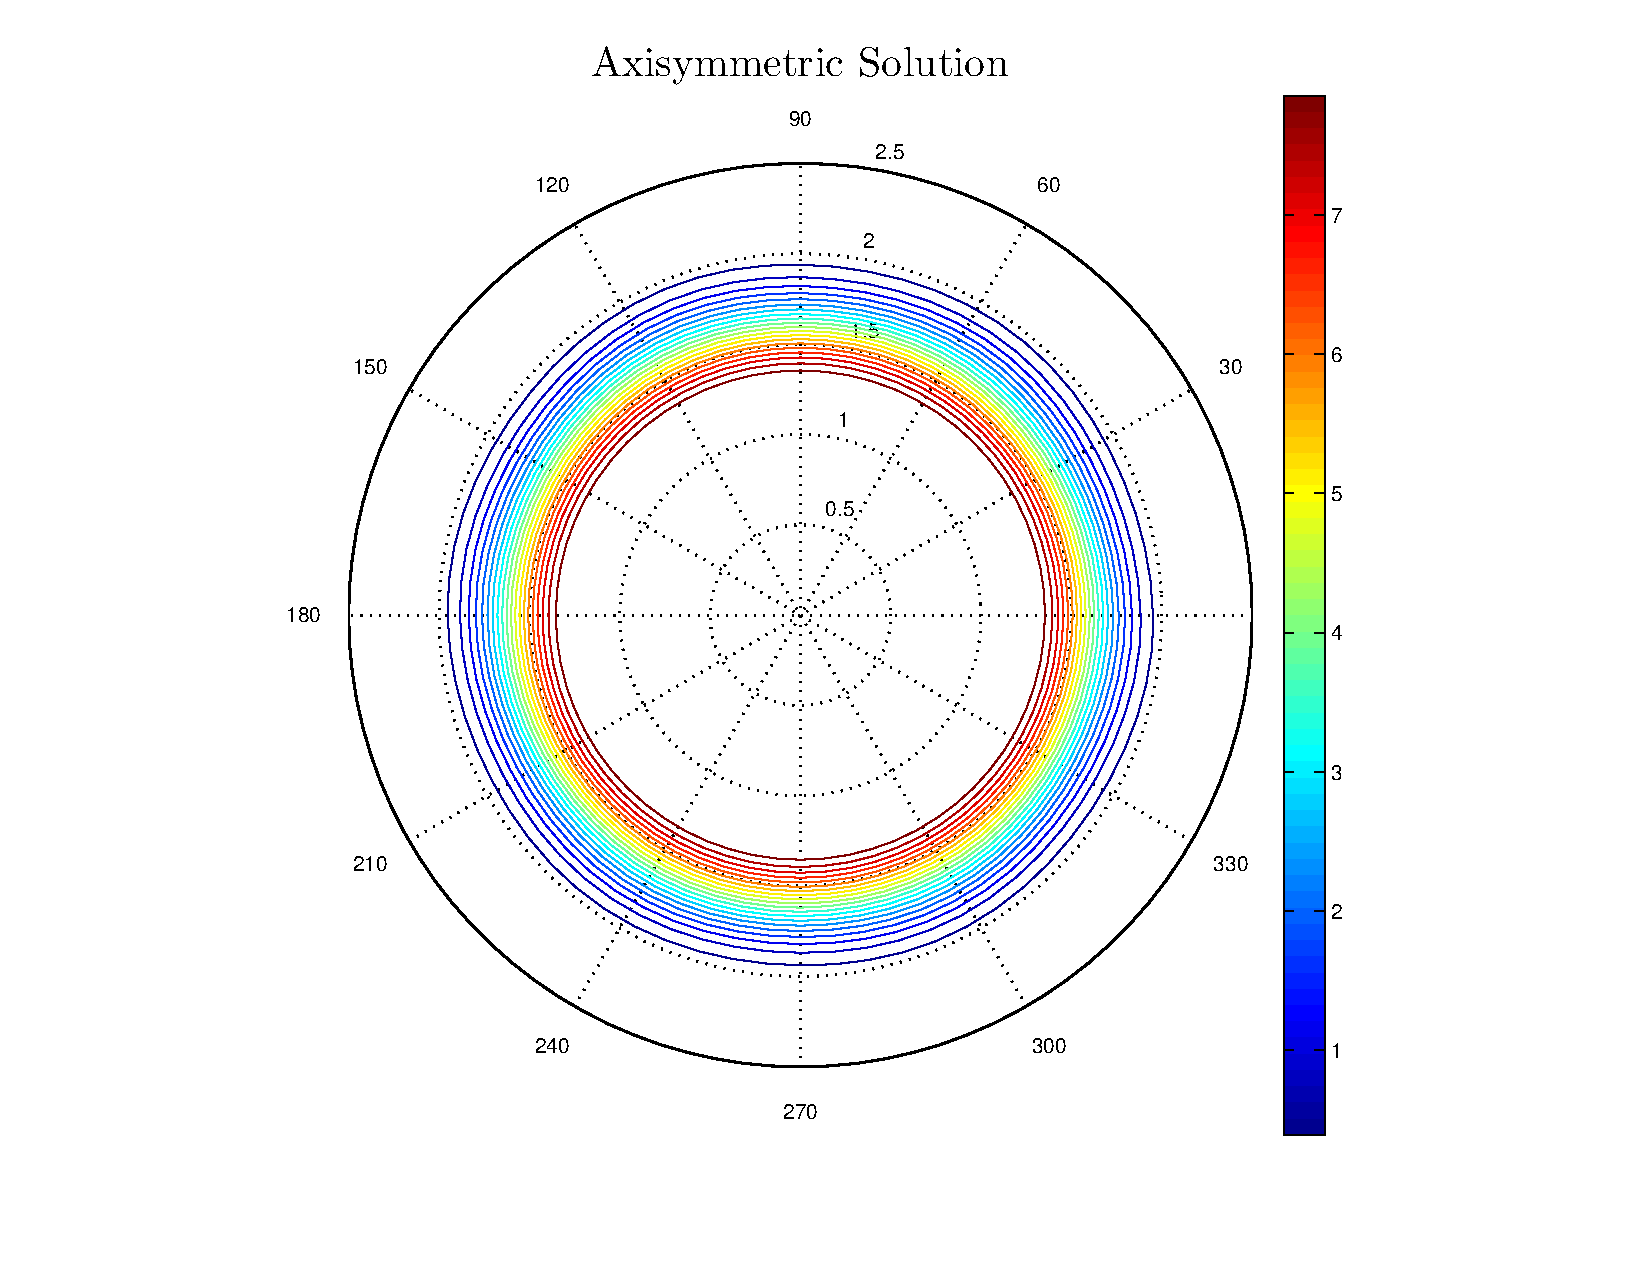
\includegraphics[width=1\textwidth, keepaspectratio]{./figures/Pictures/Axisymmetric.pdf}}
%\caption{}
%\end{figure}
%
%\subsection{Primary Transition}
%The amplitude equation for steady electroconvection in the abscence of shear describing a stationary bifurcation is reand and time independent
%\beq
%\pderiv[]{A}{t} = \epsilon A - gA|A|^2 + hA|A|^4 + f = 0
%\eeq
%where $A$ is the amplitude of the underlying fields can be computed by , with $|A|^2 = Nu - 1 = \alpha E_{kin} $ or can directly be the Fourrier amplitude of the physical field of interest. $ \epsilon = (\mathrm{Ra_c/Ra})-1$
%The first transition was shown to be supercritical Hopf bifurcation for $Pr = 10$ for a broad range $0.1 to 0.9$.
%The  values of g


%\cite{DNSSAE},\cite{linearstability},\cite{SBSAE},\cite{BAEWIS},\cite{EDCTAFUCF},\cite{ARDCTTE},
%\cite{AEWSDaDe},\cite{LSSE-PeDa}, \cite{WNAEISFF}


%Using our numerical continuation code, we have traced two branches of solution, the zero solution describing the axisymetric state and we have computed the primary transition to the rotating travelling waves which matches the results that have been investigated by the linear stability analysis as well as the time integration done. We also have trace the travelling rotating wave using the relative equilibria techniques and found another bifurcation point. We have found that the transition from axisymmetric solution to travelling rotating wave occurs at a critical Rayleigh number $R_c = 572$.
%These finding are represented in a bifurcation diagram in figure (\ref{bif_diag}).
